% Problems, Chapter 15: Bremsstrahlung, Method of Virtual Quanta, Radiative Beta Processes
% Jackson, Classical Electrodynamics, 3rd ed.
% Requires: amsmath, amssymb, tikz

\section*{Problems}

\Needspace{5\baselineskip}
\par\bigskip
\noindent\textbf{15.1}\quad In radiative collision problems it is useful to have the radiation amplitude expressed explicitly as an integral involving the accelerations of the particles, as in (14.65), for example. In the nonrelativistic limit, particles do not move rapidly or far during the period of acceleration; only the lowest order velocity and retardation effects need be kept in an approximate description.
\begin{enumerate}
\item[(a)] Show that the integral (times $e$) in (14.65), which is, apart from an inessential phase, \erratum{$\sqrt{2\pi}\,cR$ times the Fourier transform with the normalization of (14.54)} of the Li\'enard--Wiechert electric field at distance $R$, can be expanded in inverse powers of $c$ (remembering that $\beta=v/c$ and $k=\omega/c$) as follows:
\[
\mathbf{J}=e\int dt\;e^{i\omega t}(\dot{\boldsymbol{\beta}}_{\perp}+\beta_{\parallel}\dot{\boldsymbol{\beta}}_{\perp}+\dot{\beta}_{\parallel}\boldsymbol{\beta}_{\perp}-ikr_{\parallel}\dot{\boldsymbol{\beta}}_{\perp}+\cdots)
\]
or
\[
\mathbf{J}=e\int dt\;e^{i\omega t}\!\left(\dot{\boldsymbol{\beta}}_{\perp}+\frac{d}{dt}\,(\beta_{\parallel}\boldsymbol{\beta}_{\perp})-ikr_{\parallel}\dot{\boldsymbol{\beta}}_{\perp}+\cdots\right)
\]
where $\beta_{\parallel}=\boldsymbol{\beta}\cdot\mathbf{n}$, $r_{\parallel}=\mathbf{r}\cdot\mathbf{n}$, and $\boldsymbol{\beta}_{\perp}=(\mathbf{n}\times\boldsymbol{\beta})\times\mathbf{n}$. Neglected terms are of order $1/c^{3}$ and higher.
\item[(b)] Show that the first term in part a corresponds to the electric dipole approximation, while the next terms are the magnetic dipole and the electric quadrupole contributions. [Some integrations by parts are required, with a convergence factor $e^{-\epsilon|t|}$ to give meaning to the integrals, as discussed following (14.67).] For a group of charges, show that the generalization of part a can be written as
\[
\mathbf{J}=\frac{1}{c}\int dt\;e^{i\omega t}\!\left(\frac{d^{2}\mathbf{p}_{\perp}(t)}{dt^{2}}+\frac{d^{2}\mathbf{m}(t)}{dt^{2}}\times\mathbf{n}+\frac{1}{6c}\frac{d^{3}\mathbf{Q}_{\perp}}{dt^{3}}(\mathbf{n},t)+\cdots\right)
\]
and the radiated intensity per unit solid angle and per unit frequency as
\[
\frac{d^{2}I}{d\omega\;d\Omega}=\frac{1}{4\pi^{2}c^{3}}\left|\int dt\;e^{i\omega t}\!\left(\frac{d^{2}\mathbf{p}_{\perp}(t)}{dt^{2}}+\frac{d^{2}\mathbf{m}(t)}{dt^{2}}\times\mathbf{n}+\frac{1}{6c}\frac{d^{3}\mathbf{Q}_{\perp}}{dt^{3}}(\mathbf{n},t)+\cdots\right)\right|^{2}
\]
where
\[
\mathbf{p}=\sum_{j}q_{j}\mathbf{r}_{j},\qquad
\mathbf{m}=\sum_{j}q_{j}\frac{\mathbf{r}_{j}\times\boldsymbol{\beta}_{j}}{2},\qquad
Q_{\alpha\beta}=\sum_{j}q_{j}(3x_{j\alpha}x_{j\beta}-r_{j}^{2}\;\delta_{\alpha\beta})
\]
and the vector $\mathbf{Q}(\mathbf{n})$ has components, $Q_{\alpha}=\sum_{\beta}Q_{\alpha\beta}n_{\beta}$. Relate to the treatment of multipole radiation in Sections 9.2 and 9.3 and Problem 9.7.
\end{enumerate}
\solution

Use Gaussian units and let $P=\mathbf 1-\mathbf n\mathbf n^{\mathsf T}$
be the transverse projector.  Frequencies below are positive.

\medskip\noindent\textbf{(a)} The identity (14.66), checked against
(14.65), is
\[
\frac{\mathbf n\times[(\mathbf n-\boldsymbol\beta)\times
 \dot{\boldsymbol\beta}]}{(1-\beta_\parallel)^2}
=-\frac d{dt}\frac{\boldsymbol\beta_\perp}{1-\beta_\parallel}.
\]
Thus the problem's $\mathbf J$ chooses an overall minus sign relative
to the integral printed in (14.65); this is the stated inessential
phase and has no effect on intensity.  There is also a normalization
qualification in the introductory description: Jackson's transform
on p.~674, (14.54), contains $1/\sqrt{2\pi}$.  Indeed the far-zone
field and the observation-time Jacobian are
\[
\mathbf E_{\rm rad}(t_{\rm obs})
=\frac e{cR}\left[
 \frac{\mathbf n\times[(\mathbf n-\boldsymbol\beta)\times
 \dot{\boldsymbol\beta}]}{(1-\mathbf n\cdot\boldsymbol\beta)^3}
 \right]_{\rm ret},\qquad
dt_{\rm obs}=(1-\mathbf n\cdot\boldsymbol\beta)\,dt.
\]
Using $t_{\rm obs}=t+(R-\mathbf n\cdot\mathbf r)/c$ therefore gives
\[
\widetilde{\mathbf E}_{\rm rad}(\omega)
=-\frac{e^{i\omega R/c}}{\sqrt{2\pi}\,cR}\mathbf J(\omega).
\]
This explains the marked factor in the statement; the displayed
definition of $\mathbf J$ and its intensity formula need no change.
Expand the positive version of the acceleration integral:
\begin{align*}
\frac d{dt}\frac{\boldsymbol\beta_\perp}{1-\beta_\parallel}
&=\frac{\dot{\boldsymbol\beta}_\perp}{1-\beta_\parallel}
 +\frac{\boldsymbol\beta_\perp\dot\beta_\parallel}
 {(1-\beta_\parallel)^2}\\
&=\dot{\boldsymbol\beta}_\perp+
 \beta_\parallel\dot{\boldsymbol\beta}_\perp+
 \dot\beta_\parallel\boldsymbol\beta_\perp+O(c^{-3}),\\
e^{-ikr_\parallel}&=1-ikr_\parallel+O(c^{-2}).
\end{align*}
The leading acceleration is already $O(c^{-1})$.  Multiplication
therefore gives
\[
\boxed{\mathbf J=e\int e^{i\omega t}
 [\dot{\boldsymbol\beta}_\perp+
 (\beta_\parallel\boldsymbol\beta_\perp)^{\displaystyle\cdot}
 -ikr_\parallel\dot{\boldsymbol\beta}_\perp]dt+O(c^{-3}).}
\]
The expansion requires both $v/c\ll1$ and small source displacement
in units of $c/\omega$ during the acceleration.  It does not require
an eternally unbounded straight trajectory to fit inside a wavelength.

\medskip\noindent\textbf{(b)} Put $b=r_\parallel$ and
$\mathbf a=\mathbf r_\perp$ temporarily.  The second-order integral
is
\[
\frac e{c^2}\int e^{i\omega t}
 [(\dot b\dot{\mathbf a})^{\displaystyle\cdot}
 -i\omega b\ddot{\mathbf a}]dt.
\]
Insert $e^{-\epsilon|t|}$ and integrate by parts before taking
$\epsilon\downarrow0$.  For $\omega>0$ the boundary terms vanish
in this regulated sense, and
\[
\int e^{i\omega t}(-i\omega)b\ddot{\mathbf a}\,dt
=\int e^{i\omega t}(\dot b\ddot{\mathbf a}
+b\dddot{\mathbf a})dt.
\]
The resulting integrand is
$e[\ddot b\dot{\mathbf a}+2\dot b\ddot{\mathbf a}
+b\dddot{\mathbf a}]/c^2$.
For one charge the definitions in the question give
\[
\mathbf m\times\mathbf n=\frac e{2c}
 (b\dot{\mathbf a}-\dot b\mathbf a),\qquad
\mathbf Q_\perp=3eb\mathbf a.
\]
Differentiate both products explicitly:
\begin{align*}
(b\dot{\mathbf a}-\dot b\mathbf a)''
 &=b\dddot{\mathbf a}+\dot b\ddot{\mathbf a}
  -\ddot b\dot{\mathbf a}-\dddot b\mathbf a,\\
(b\mathbf a)'''&=b\dddot{\mathbf a}+3\dot b\ddot{\mathbf a}
 +3\ddot b\dot{\mathbf a}+\dddot b\mathbf a.
\end{align*}
Their sum proves
\[
\frac1c\left(\ddot{\mathbf m}\times\mathbf n+
 \frac{\dddot{\mathbf Q}_\perp}{6c}\right)
=\frac e{c^2}(b\dddot{\mathbf a}+2\dot b\ddot{\mathbf a}
+\ddot b\dot{\mathbf a}).
\]
Also $e\dot{\boldsymbol\beta}_\perp=\ddot{\mathbf p}_\perp/c$.
Adding the amplitudes of all charges, before squaring, yields
\[
\boxed{\mathbf J=\frac1c\int e^{i\omega t}
 \left(\ddot{\mathbf p}_\perp+\ddot{\mathbf m}\times\mathbf n
 +\frac{\dddot{\mathbf Q}_\perp}{6c}\right)dt+O(c^{-3}),}
\]
and $d^2I/(d\omega\,d\Omega)=|\mathbf J|^2/(4\pi^2c)$ gives
the stated intensity.  These are precisely the electric dipole,
magnetic dipole and traceless electric quadrupole moments of
Sections 9.2--9.3.  For a Fourier component their derivatives
supply $-\omega^2,-\omega^2,i\omega^3$, respectively; the last
coefficient includes the $1/6$ appropriate to the definition
$Q_{ij}=\sum q(3x_ix_j-r^2\delta_{ij})$.  These are the
time-domain forms of Problem 9.7 (in SI there): its replacement of
$(\mathbf n\times\ddot{\mathbf p})\times\mathbf n$ by
$\ddot{\mathbf m}\times\mathbf n/c$ becomes
$\ddot{\mathbf m}\times\mathbf n$ here, because the Gaussian
$\mathbf m$ above already contains $1/c$; the coefficient ratio
$16/576=1/6^2$ there corresponds to the amplitude
$\dddot{\mathbf Q}_\perp/(6c)$.  Here the three amplitudes
add coherently, so their square also contains interference terms.
No monopole term occurs because the total charge is constant.

\Needspace{5\baselineskip}
\par\bigskip
\noindent\textbf{15.2}\quad A nonrelativistic particle of charge $e$ and mass $m$ collides with a fixed, smooth, hard sphere of radius $R$. Assuming that the collision is elastic, show that in the dipole approximation (neglecting retardation effects) the classical differential cross section for the emission of photons per unit solid angle per unit energy interval is
\[
\frac{d^{2}\sigma}{d\Omega\;d(\hbar\omega)}=\frac{R^{2}}{12\pi}\frac{e^{2}}{\hbar c}\left(\frac{v}{c}\right)^{2}\frac{1}{\hbar\omega}\,(2+3\sin^{2}\theta)
\]
where $\theta$ is measured relative to the incident direction. Sketch the angular distribution. Integrate over angles to get the total bremsstrahlung cross section. Qualitatively, what factor (or factors) govern the upper limit to the frequency spectrum?
\solution

Let $\varepsilon=\hbar\omega$, $\alpha=e^2/(\hbar c)$,
$\boldsymbol\beta=\beta\widehat{\mathbf z}$ and let
$\mathbf u$ be the outgoing velocity direction.  If $\chi$ is the
particle's scattering angle, specular reflection gives
$b=R\cos(\chi/2)$.  Consequently
\[
 d\sigma_{\rm el}=b|db|\,d\phi
 =\frac{R^2}4\sin\chi\,d\chi\,d\phi
 =\frac{R^2}4d\Omega_{\mathbf u}.
\]
The soft dipole photon probability for this one collision is
\[
\frac{d^2N}{d\varepsilon\,d\Omega}
=\frac{\alpha\beta^2}{4\pi^2\varepsilon}
 |P(\mathbf u-\widehat{\mathbf z})|^2,
\qquad P=\mathbf1-\mathbf n\mathbf n^{\mathsf T}.
\]
The average over outgoing directions uses
$\langle u_i\rangle=0$, $\langle u_iu_j\rangle=\delta_{ij}/3$.
It follows that
\[
\langle|P\mathbf u|^2\rangle=\tfrac23,\qquad
|P\widehat{\mathbf z}|^2=\sin^2\theta,\qquad
\langle P\mathbf u\cdot P\widehat{\mathbf z}\rangle=0.
\]
Multiplication by the total elastic area $\pi R^2$ gives
\[
\boxed{\frac{d^2\sigma}{d\Omega\,d\varepsilon}
 =\frac{\alpha\beta^2R^2}{12\pi\varepsilon}
 (2+3\sin^2\theta).}
\]
The distribution is independent of azimuth, symmetric forward and
backward, and has maximum-to-minimum ratio $5/2$.  The following
polar sketch uses radius proportional to $2+3\sin^2\theta$ and a
horizontal incident direction.
\begin{center}% Generated by supplementary/check_ch15.py
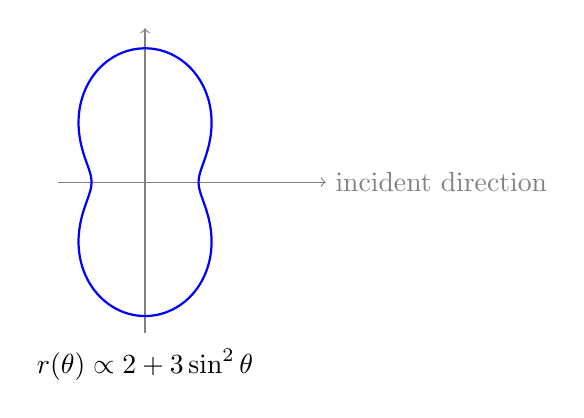
\begin{tikzpicture}[scale=0.85]
\draw[->,gray] (-1.3,0)--(2.7,0) node[right] {incident direction};
\draw[->,gray] (0,-2.25)--(0,2.3);
\draw[blue,thick] plot coordinates {(0.8,0) (0.800244,0.0139683) (0.800973,0.0279706) (0.802186,0.0420408) (0.803876,0.0562125) (0.806036,0.070519) (0.808657,0.0849933) (0.811727,0.0996675) (0.815231,0.114573) (0.819155,0.129741) (0.823481,0.145202) (0.828189,0.160984) (0.833257,0.177114) (0.838663,0.193621) (0.844382,0.210528) (0.850386,0.22786) (0.856649,0.24564) (0.863139,0.263888) (0.869827,0.282624) (0.876679,0.301865) (0.883662,0.321627) (0.890741,0.341924) (0.897881,0.362768) (0.905045,0.384169) (0.912195,0.406135) (0.919293,0.428673) (0.9263,0.451787) (0.933177,0.475477) (0.939884,0.499745) (0.946381,0.524587) (0.952628,0.55) (0.958585,0.575976) (0.964211,0.602506) (0.969468,0.62958) (0.974315,0.657184) (0.978713,0.685302) (0.982624,0.713918) (0.986009,0.743011) (0.988833,0.772561) (0.991058,0.802543) (0.992649,0.832931) (0.993572,0.863699) (0.993795,0.894817) (0.993285,0.926253) (0.992013,0.957976) (0.989949,0.989949) (0.987068,1.02214) (0.983342,1.05451) (0.978749,1.08701) (0.973266,1.11961) (0.966874,1.15228) (0.959554,1.18495) (0.951291,1.2176) (0.942071,1.25017) (0.931881,1.28262) (0.920712,1.31491) (0.908556,1.34699) (0.895409,1.37881) (0.881268,1.41032) (0.866131,1.44148) (0.85,1.47224) (0.832879,1.50255) (0.814775,1.53237) (0.795696,1.56164) (0.775653,1.59032) (0.754658,1.61837) (0.732727,1.64573) (0.709878,1.67237) (0.686131,1.69823) (0.661507,1.72328) (0.63603,1.74748) (0.609726,1.77077) (0.582624,1.79313) (0.554753,1.81451) (0.526145,1.83488) (0.496833,1.85421) (0.466853,1.87245) (0.436242,1.88957) (0.405038,1.90556) (0.373282,1.92037) (0.341013,1.93398) (0.308275,1.94637) (0.275111,1.95752) (0.241567,1.9674) (0.207686,1.976) (0.173517,1.98331) (0.139106,1.9893) (0.1045,1.99398) (0.069748,1.99732) (0.0348984,1.99933) (1.22465e-16,2) (-0.0348984,1.99933) (-0.069748,1.99732) (-0.1045,1.99398) (-0.139106,1.9893) (-0.173517,1.98331) (-0.207686,1.976) (-0.241567,1.9674) (-0.275111,1.95752) (-0.308275,1.94637) (-0.341013,1.93398) (-0.373282,1.92037) (-0.405038,1.90556) (-0.436242,1.88957) (-0.466853,1.87245) (-0.496833,1.85421) (-0.526145,1.83488) (-0.554753,1.81451) (-0.582624,1.79313) (-0.609726,1.77077) (-0.63603,1.74748) (-0.661507,1.72328) (-0.686131,1.69823) (-0.709878,1.67237) (-0.732727,1.64573) (-0.754658,1.61837) (-0.775653,1.59032) (-0.795696,1.56164) (-0.814775,1.53237) (-0.832879,1.50255) (-0.85,1.47224) (-0.866131,1.44148) (-0.881268,1.41032) (-0.895409,1.37881) (-0.908556,1.34699) (-0.920712,1.31491) (-0.931881,1.28262) (-0.942071,1.25017) (-0.951291,1.2176) (-0.959554,1.18495) (-0.966874,1.15228) (-0.973266,1.11961) (-0.978749,1.08701) (-0.983342,1.05451) (-0.987068,1.02214) (-0.989949,0.989949) (-0.992013,0.957976) (-0.993285,0.926253) (-0.993795,0.894817) (-0.993572,0.863699) (-0.992649,0.832931) (-0.991058,0.802543) (-0.988833,0.772561) (-0.986009,0.743011) (-0.982624,0.713918) (-0.978713,0.685302) (-0.974315,0.657184) (-0.969468,0.62958) (-0.964211,0.602506) (-0.958585,0.575976) (-0.952628,0.55) (-0.946381,0.524587) (-0.939884,0.499745) (-0.933177,0.475477) (-0.9263,0.451787) (-0.919293,0.428673) (-0.912195,0.406135) (-0.905045,0.384169) (-0.897881,0.362768) (-0.890741,0.341924) (-0.883662,0.321627) (-0.876679,0.301865) (-0.869827,0.282624) (-0.863139,0.263888) (-0.856649,0.24564) (-0.850386,0.22786) (-0.844382,0.210528) (-0.838663,0.193621) (-0.833257,0.177114) (-0.828189,0.160984) (-0.823481,0.145202) (-0.819155,0.129741) (-0.815231,0.114573) (-0.811727,0.0996675) (-0.808657,0.0849933) (-0.806036,0.070519) (-0.803876,0.0562125) (-0.802186,0.0420408) (-0.800973,0.0279706) (-0.800244,0.0139683) (-0.8,9.79717e-17) (-0.800244,-0.0139683) (-0.800973,-0.0279706) (-0.802186,-0.0420408) (-0.803876,-0.0562125) (-0.806036,-0.070519) (-0.808657,-0.0849933) (-0.811727,-0.0996675) (-0.815231,-0.114573) (-0.819155,-0.129741) (-0.823481,-0.145202) (-0.828189,-0.160984) (-0.833257,-0.177114) (-0.838663,-0.193621) (-0.844382,-0.210528) (-0.850386,-0.22786) (-0.856649,-0.24564) (-0.863139,-0.263888) (-0.869827,-0.282624) (-0.876679,-0.301865) (-0.883662,-0.321627) (-0.890741,-0.341924) (-0.897881,-0.362768) (-0.905045,-0.384169) (-0.912195,-0.406135) (-0.919293,-0.428673) (-0.9263,-0.451787) (-0.933177,-0.475477) (-0.939884,-0.499745) (-0.946381,-0.524587) (-0.952628,-0.55) (-0.958585,-0.575976) (-0.964211,-0.602506) (-0.969468,-0.62958) (-0.974315,-0.657184) (-0.978713,-0.685302) (-0.982624,-0.713918) (-0.986009,-0.743011) (-0.988833,-0.772561) (-0.991058,-0.802543) (-0.992649,-0.832931) (-0.993572,-0.863699) (-0.993795,-0.894817) (-0.993285,-0.926253) (-0.992013,-0.957976) (-0.989949,-0.989949) (-0.987068,-1.02214) (-0.983342,-1.05451) (-0.978749,-1.08701) (-0.973266,-1.11961) (-0.966874,-1.15228) (-0.959554,-1.18495) (-0.951291,-1.2176) (-0.942071,-1.25017) (-0.931881,-1.28262) (-0.920712,-1.31491) (-0.908556,-1.34699) (-0.895409,-1.37881) (-0.881268,-1.41032) (-0.866131,-1.44148) (-0.85,-1.47224) (-0.832879,-1.50255) (-0.814775,-1.53237) (-0.795696,-1.56164) (-0.775653,-1.59032) (-0.754658,-1.61837) (-0.732727,-1.64573) (-0.709878,-1.67237) (-0.686131,-1.69823) (-0.661507,-1.72328) (-0.63603,-1.74748) (-0.609726,-1.77077) (-0.582624,-1.79313) (-0.554753,-1.81451) (-0.526145,-1.83488) (-0.496833,-1.85421) (-0.466853,-1.87245) (-0.436242,-1.88957) (-0.405038,-1.90556) (-0.373282,-1.92037) (-0.341013,-1.93398) (-0.308275,-1.94637) (-0.275111,-1.95752) (-0.241567,-1.9674) (-0.207686,-1.976) (-0.173517,-1.98331) (-0.139106,-1.9893) (-0.1045,-1.99398) (-0.069748,-1.99732) (-0.0348984,-1.99933) (-3.67394e-16,-2) (0.0348984,-1.99933) (0.069748,-1.99732) (0.1045,-1.99398) (0.139106,-1.9893) (0.173517,-1.98331) (0.207686,-1.976) (0.241567,-1.9674) (0.275111,-1.95752) (0.308275,-1.94637) (0.341013,-1.93398) (0.373282,-1.92037) (0.405038,-1.90556) (0.436242,-1.88957) (0.466853,-1.87245) (0.496833,-1.85421) (0.526145,-1.83488) (0.554753,-1.81451) (0.582624,-1.79313) (0.609726,-1.77077) (0.63603,-1.74748) (0.661507,-1.72328) (0.686131,-1.69823) (0.709878,-1.67237) (0.732727,-1.64573) (0.754658,-1.61837) (0.775653,-1.59032) (0.795696,-1.56164) (0.814775,-1.53237) (0.832879,-1.50255) (0.85,-1.47224) (0.866131,-1.44148) (0.881268,-1.41032) (0.895409,-1.37881) (0.908556,-1.34699) (0.920712,-1.31491) (0.931881,-1.28262) (0.942071,-1.25017) (0.951291,-1.2176) (0.959554,-1.18495) (0.966874,-1.15228) (0.973266,-1.11961) (0.978749,-1.08701) (0.983342,-1.05451) (0.987068,-1.02214) (0.989949,-0.989949) (0.992013,-0.957976) (0.993285,-0.926253) (0.993795,-0.894817) (0.993572,-0.863699) (0.992649,-0.832931) (0.991058,-0.802543) (0.988833,-0.772561) (0.986009,-0.743011) (0.982624,-0.713918) (0.978713,-0.685302) (0.974315,-0.657184) (0.969468,-0.62958) (0.964211,-0.602506) (0.958585,-0.575976) (0.952628,-0.55) (0.946381,-0.524587) (0.939884,-0.499745) (0.933177,-0.475477) (0.9263,-0.451787) (0.919293,-0.428673) (0.912195,-0.406135) (0.905045,-0.384169) (0.897881,-0.362768) (0.890741,-0.341924) (0.883662,-0.321627) (0.876679,-0.301865) (0.869827,-0.282624) (0.863139,-0.263888) (0.856649,-0.24564) (0.850386,-0.22786) (0.844382,-0.210528) (0.838663,-0.193621) (0.833257,-0.177114) (0.828189,-0.160984) (0.823481,-0.145202) (0.819155,-0.129741) (0.815231,-0.114573) (0.811727,-0.0996675) (0.808657,-0.0849933) (0.806036,-0.070519) (0.803876,-0.0562125) (0.802186,-0.0420408) (0.800973,-0.0279706) (0.800244,-0.0139683) (0.8,-1.95943e-16)};
\node[below] at (0,-2.35) {$r(\theta)\propto2+3\sin^2\theta$};
\end{tikzpicture}
\end{center}
Because $\int d\Omega=4\pi$ and
$\int\sin^2\theta\,d\Omega=8\pi/3$,
\[
\boxed{\frac{d\sigma}{d\varepsilon}
=\frac{4\alpha R^2\beta^2}{3\varepsilon}.}
\]
On a photon-energy band $[\varepsilon_1,\varepsilon_2]$ this gives
$\sigma=(4/3)\alpha R^2\beta^2\ln(\varepsilon_2/\varepsilon_1)$.
Its number integral has the familiar infrared divergence if the
lower limit is set to zero, whereas its energy integral is finite.
An ideal instantaneous hard collision has no classical high-frequency
cutoff.  For a real interaction, a collision duration $\tau$ produces
loss of coherence for $\omega\tau\gtrsim1$; the range over which
the force changes sets $\tau$.  Energy conservation additionally
requires $\varepsilon\leq mv^2/2$ (a massive fixed scatterer absorbs
momentum with negligible recoil energy).  The dipole and soft
formulas should be used below both scales, not extrapolated as exact
spectra at their endpoint.

\Needspace{5\baselineskip}
\par\bigskip
\noindent\textbf{15.3}\quad Treat Problem 15.2 without the assumption of nonrelativistic motion, using (15.2) and assuming the elastic impact is of negligible duration. Show that the cross section for photon emission is now
\[
\frac{d^{2}\sigma}{d\Omega\;d(\hbar\omega)}=\frac{R^{2}}{4\pi}\frac{e^{2}}{\hbar c}\frac{\beta^{2}}{\hbar\omega}\left[\frac{\sin^{2}\theta}{(1-\beta\cos\theta)^{2}}+\frac{1}{\beta^{3}}\ln\!\left(\frac{1+\beta}{1-\beta}\right)-\frac{2}{\beta^{2}}\right]
\]
\solution

The elastic angular distribution remains $d\sigma_{\rm el}
=(R^2/4)d\Omega_{\mathbf u}$: it is a geometrical consequence of
specular reflection, independent of speed.  Equation (15.2) gives
\[
\frac{d^2\sigma}{d\Omega\,d\varepsilon}
=\frac{\alpha R^2}{16\pi^2\varepsilon}
\int d\Omega_{\mathbf u}\left|
 \frac{\beta P\mathbf u}{1-\beta\mathbf n\cdot\mathbf u}
 -\frac{\beta P\widehat{\mathbf z}}{1-\beta\cos\theta}
\right|^2.
\]
The angular average of the first vector is zero: rotation about
$\mathbf n$ leaves only a vector parallel to $\mathbf n$, and $P$
removes that component.  Thus the cross term vanishes.  Set
$t=\mathbf n\cdot\mathbf u$.  The first squared term is
\[
2\pi\beta^2\int_{-1}^{1}\frac{1-t^2}{(1-\beta t)^2}\,dt.
\]
With $y=1-\beta t$ its integral becomes
\begin{align*}
\int_{-1}^{1}\frac{1-t^2}{(1-\beta t)^2}\,dt
&=\frac1{\beta^3}\int_{1-\beta}^{1+\beta}
 \left[\frac{\beta^2-1}{y^2}+\frac2y-1\right]dy\\
&=\frac2{\beta^3}\ln\frac{1+\beta}{1-\beta}
 -\frac4{\beta^2}.
\end{align*}
The second squared term integrates to
$4\pi\beta^2\sin^2\theta/(1-\beta\cos\theta)^2$.
Therefore
\[
\boxed{\frac{d^2\sigma}{d\Omega\,d\varepsilon}
=\frac{\alpha R^2\beta^2}{4\pi\varepsilon}
\left[\frac{\sin^2\theta}{(1-\beta\cos\theta)^2}
 +\frac1{\beta^3}\ln\frac{1+\beta}{1-\beta}
 -\frac2{\beta^2}\right].}
\]
As a check, the apparent small-$\beta$ singularity cancels because
$\ln[(1+\beta)/(1-\beta)]=2\beta+2\beta^3/3+\cdots$.
The bracket becomes $\sin^2\theta+2/3$, recovering Problem 15.2.
Integration over the photon direction gives the useful further check
\[
\frac{d\sigma}{d\varepsilon}
=\frac{2\alpha R^2}{\varepsilon}
\left[\frac1\beta\ln\frac{1+\beta}{1-\beta}-2\right].
\]
The instantaneous-impact assumption removes the classical duration
cutoff; it does not remove the soft-photon restriction implicit in
using an elastic trajectory at unchanged particle energy.

\Needspace{5\baselineskip}
\par\bigskip
\noindent\textbf{15.4}\quad A group of charged particles with charges $e_{j}$ and coordinates $\mathbf{r}_{j}(t)$ undergo interactions and are accelerated only during a time $-\tau/2<t<\tau/2$, during which their velocities change from $c\boldsymbol{\beta}_{j}$ to $c\boldsymbol{\beta}'_{j}$.
\begin{enumerate}
\item[(a)] Show that for $\omega\tau\ll1$ the intensity of radiation emitted with polarization $\boldsymbol{\epsilon}$ per unit solid angle and unit frequency interval is
\[
\frac{d^{2}I}{d\omega\;d\Omega}=\frac{1}{4\pi^{2}c}\,|\boldsymbol{\epsilon}^{*}\cdot\mathbf{E}|^{2}
\]
where
\[
\mathbf{E}=\sum_{j}e_{j}\!\left(\frac{\boldsymbol{\beta}'_{j}}{1-\mathbf{n}\cdot\boldsymbol{\beta}'_{j}}-\frac{\boldsymbol{\beta}_{j}}{1-\mathbf{n}\cdot\boldsymbol{\beta}_{j}}\right)\!e^{-i\omega\mathbf{n}\cdot\mathbf{r}_{j}(0)/c}
\]
\item[(b)] An $\omega^{0}$ meson of mass 784 MeV decays into $\pi^{+}\pi^{-}$ and $e^{+}e^{-}$ with branching ratios of $1.3\times10^{-2}$ and $8\times10^{-5}$, respectively. Show that for both decay modes the frequency spectrum of radiated energy at low frequencies is
\[
\frac{dI}{d\omega}=\frac{e^{2}}{\pi c}\left[\left(\frac{1+\beta^{2}}{\beta}\right)\ln\!\left(\frac{1+\beta}{1-\beta}\right)-2\right]\simeq\frac{4e^{2}}{\pi c}\left[\ln\!\left(\frac{M_{\omega}}{m}\right)-\frac{1}{2}\right]
\]
where $M_{\omega}$ is the mass of the $\omega^{0}$ meson and $m$ is the mass of one of the decay products. Evaluate approximately the \emph{total} energy radiated in each decay by integrating the spectrum up to the maximum frequency allowed kinematically. What fraction of the rest energy of the $\omega^{0}$ is it in each decay?
\end{enumerate}
\solution

\medskip\noindent\textbf{(a)} For each charge use the derivative
identity (14.66), with the common overall sign chosen as in
Problem 15.1.  During acceleration,
\[
\omega[t-\mathbf n\cdot\mathbf r_j(t)/c]
=-\omega\mathbf n\cdot\mathbf r_j(0)/c+O(\omega\tau),
\]
since $|\mathbf r_j(t)-\mathbf r_j(0)|\leq c|t|$.
Thus the phase can be pulled out of its acceleration integral and
\[
\int dt\,\frac d{dt}\frac{\boldsymbol\beta_j}
 {1-\mathbf n\cdot\boldsymbol\beta_j}
=\frac{\boldsymbol\beta'_j}{1-\mathbf n\cdot\boldsymbol\beta'_j}
 -\frac{\boldsymbol\beta_j}{1-\mathbf n\cdot\boldsymbol\beta_j}.
\]
Summing the amplitudes proves exactly the stated $\mathbf E$ and
$d^2I/(d\omega\,d\Omega)=|\boldsymbol\epsilon^*\cdot\mathbf E|^2/
(4\pi^2c)$, to leading order in $\omega\tau$.  The fixed positions
need not be mutually close compared with a wavelength; their relative
phases have deliberately been retained.  Polarization vectors satisfy
$\boldsymbol\epsilon\cdot\mathbf n=0$.

\medskip\noindent\textbf{(b)} In the parent rest frame the two
opposite charges are created at the same event with velocities
$\pm c\beta\widehat{\mathbf z}$, where
$\beta=\sqrt{1-4m^2/M_\omega^2}$.  The neutral parent contributes
no endpoint term, so
\[
\mathbf E=\frac{2e\beta\widehat{\mathbf z}}
 {1-\beta^2\cos^2\theta},\qquad
\frac{d^2I}{d\omega\,d\Omega}
=\frac{e^2\beta^2}{\pi^2c}
\frac{1-\cos^2\theta}{(1-\beta^2\cos^2\theta)^2}.
\]
To integrate, write $L=\ln[(1+\beta)/(1-\beta)]$ and use
\[
\frac{1-x^2}{(1-\beta^2x^2)^2}
=\frac{\beta^2-1}{2\beta^2}
 \frac d{dx}\frac{x}{1-\beta^2x^2}
+\frac{\beta^2+1}{2\beta^2}\frac1{1-\beta^2x^2}.
\]
The two elementary endpoint integrals give
\[
\int_{-1}^1\frac{1-x^2}{(1-\beta^2x^2)^2}dx
=-\frac1{\beta^2}+\frac{1+\beta^2}{2\beta^3}L.
\]
Multiplying by $2\pi e^2\beta^2/(\pi^2c)$ proves
\[
\boxed{\frac{dI}{d\omega}=
\frac{e^2}{\pi c}\left[\frac{1+\beta^2}{\beta}L-2\right].}
\]
For $m\ll M_\omega$, $1-\beta\simeq2m^2/M_\omega^2$,
$L\simeq2\ln(M_\omega/m)$ and $(1+\beta^2)/\beta\simeq2$,
which gives the stated approximation.

For the requested endpoint estimate set
$C=(1/\hbar)dI/d\omega=dI/d\varepsilon$.  The remaining pair has
invariant mass at least $2m$, and hence
\[
(M_\omega c^2-\varepsilon)^2-\varepsilon^2\geq(2mc^2)^2,
\qquad
\varepsilon_{\max}=\frac{M_\omega^2-4m^2}{2M_\omega}c^2.
\]
Using this endpoint rather than $ (M_\omega-2m)c^2$ is necessary
because the pair must balance the photon momentum.  Holding the soft
coefficient fixed gives $I_{\rm est}=C\varepsilon_{\max}$:
\begin{center}
\begin{tabular}{lrrrr}
\toprule
Mode&$\beta$&$\varepsilon_{\max}$ (MeV)&$I_{\rm est}$ (MeV)&$I_{\rm est}/M_\omega c^2$\\
\midrule
$\pi^+\pi^-$&0.934439&342.285&3.8042&$4.8523\times10^{-3}$\\
$e^+e^-$&0.99999915&391.999&24.897&$3.1757\times10^{-2}$\\
\bottomrule
\end{tabular}
\end{center}
Here $m_\pi c^2=139.6$ MeV, $m_ec^2=0.510999$ MeV and
$\alpha^{-1}=137.036$ were used.  These are energies per decay in
the indicated channel.  Multiplication by the stated branching ratios
gives contributions $0.04945$ and $0.001992$ MeV per parent decay
averaged over all channels.  The endpoint extrapolation is only the
rough estimate requested: recoil changes the daughter velocities and
phase space, so a constant soft spectrum is not a controlled
prediction at $\varepsilon\sim\varepsilon_{\max}$.

\Needspace{5\baselineskip}
\par\bigskip
\noindent\textbf{15.5}\quad A situation closely related to that of Problem 15.4b is the emission of radiation caused by the disappearance of charges and magnetic moments in the annihilation of electrons and positrons to form hadrons in high-energy storage ring experiments. If the differential cross section for the process $e^{+}e^{-}\to$ hadrons is $d\sigma_{0}$, \emph{without} the emission of photons, calculate the cross section for the same process accompanied by a \emph{soft} photon ($\hbar\omega\to0$) in the energy interval $d(\hbar\omega)$ around $\hbar\omega$. Compare your results with the quantum-mechanical expressions:
\begin{gather*}
\frac{d^{2}\sigma}{d\Omega\;d(\hbar\omega)}=\frac{\alpha}{\pi^{2}}\frac{d\sigma_{0}(s')}{\hbar\omega}\sqrt{\frac{s'^{2}-4m^{2}s'}{s^{2}-4m^{2}s}}\;
\cdot\frac{\left[\beta^{2}\sin^{2}\theta+\dfrac{\hbar^{2}\omega^{2}}{s'+2m^{2}}\,(1-\beta^{4}\cos^{4}\theta)\right]}{(1-\beta^{2}\cos^{2}\theta)^{2}}\\[8pt]
\frac{d\sigma}{d(\hbar\omega)}=\frac{4\alpha}{\pi}\frac{d\sigma_{0}(s')}{\hbar\omega}\sqrt{\frac{s'^{2}-4m^{2}s'}{s^{2}-4m^{2}s}}\;
\left\{\frac{1}{2}\left[\frac{1+\beta^{2}}{2\beta}\ln\!\left(\frac{1+\beta}{1-\beta}\right)-1\right]\right.\\[6pt]
\left.+\;\frac{\hbar^{2}\omega^{2}}{s'+2m^{2}}\left[\frac{1}{\beta}\ln\!\left(\frac{1+\beta}{1-\beta}\right)-1\right]\right\}
\end{gather*}
where $s=(p_{1}+p_{2})^{2}$, $s'=(p_{1}+p_{2}-k)^{2}$, $\beta=$ electron $v/c$ in c.m.\ frame. Neglect the emission of radiation by any of the hadrons, all assumed to be much heavier than the electrons.

The factors proportional to $\omega^{2}$ in the numerators of these expressions can be attributed to the disappearance of the magnetic moments. If you have not included such contributions in your semiclassical calculation, you may consider doing so.
\solution

Write $\varepsilon=\hbar\omega$ and use the center-of-mass frame.
The incoming electron and positron have opposite velocities
$\pm c\beta\widehat{\mathbf z}$; their disappearance reverses the
amplitude in Problem 15.4 but not its square.  Under the stipulated
neglect of hadron radiation, the probability of a soft photon
factorizes from the nonradiative process:
\[
\boxed{\frac{d^2\sigma}{d\Omega\,d\varepsilon}
=d\sigma_0(s)\frac{\alpha}{\pi^2\varepsilon}
 \frac{\beta^2\sin^2\theta}{(1-\beta^2\cos^2\theta)^2}.}
\]
This is a cross section still differential in whatever hadronic
variables are represented by $d\sigma_0$.  The angular integral
already evaluated in Problem 15.4 gives
\[
\boxed{\frac{d\sigma}{d\varepsilon}
=d\sigma_0(s)\frac{\alpha}{\pi\varepsilon}
 \left[\frac{1+\beta^2}{\beta}
 \ln\frac{1+\beta}{1-\beta}-2\right].}
\]
For ultrarelativistic incident beams this becomes
$(4\alpha/\pi\varepsilon)d\sigma_0(s)
[\ln(\sqrt{s}/m)-1/2]$, with energies and masses in common units.
A finite photon-energy band gives this coefficient times
$\ln(\varepsilon_2/\varepsilon_1)$.

To compare term by term with the supplied quantum result, note that
$s'=s-2\sqrt{s}\varepsilon$ in units $c=1$.  Thus
$d\sigma_0(s')\to d\sigma_0(s)$ and
\[
\sqrt{\frac{s'^2-4m^2s'}{s^2-4m^2s}}\longrightarrow1,
\qquad \frac{\varepsilon^2}{s'+2m^2}\longrightarrow0.
\]
The entire coefficient of $1/\varepsilon$, both angular and
integrated, agrees.  In particular the first term in the braces of
the quantum integrated expression equals
$[(1+\beta^2)L/\beta-2]/4$, where
$L=\ln[(1+\beta)/(1-\beta)]$.

A sudden disappearance of a magnetic moment gives a Fourier
amplitude proportional to $\omega\mathbf m$, in contrast to the
constant electric-charge endpoint amplitude.  Its intensity is
therefore $O(\omega^2)$ and its photon spectrum is $O(\varepsilon)$.
It does not modify the soft answer.  The angular function of the
quoted magnetic contribution can be checked without assuming an
unprovided classical spin ensemble:
\begin{align*}
\int d\Omega\,\frac{1-\beta^4\cos^4\theta}
 {(1-\beta^2\cos^2\theta)^2}
&=2\pi\int_{-1}^{1}\left[\frac2{1-\beta^2x^2}-1\right]dx\\
&=4\pi\left(\frac L\beta-1\right).
\end{align*}
This reproduces the second term of the supplied integrated formula.
Its precise coefficient $1/(s'+2m^2)$ describes spin and the
annihilation process beyond the universal soft approximation; the
spinless endpoint calculation by itself does not determine it.
Likewise recoil and the variation of $d\sigma_0(s')$ cannot be
inferred by extending a strictly soft classical trajectory.

\Needspace{5\baselineskip}
\par\bigskip
\noindent\textbf{15.6}\quad For the soft-photon limit of radiation emitted when there is a small change $\Delta\boldsymbol{\beta}$ of velocity, (15.9) applies, with convenient polarization vectors shown in Fig.~15.2.
\begin{enumerate}
\item[(a)] Show that
\begin{align*}
\boldsymbol{\epsilon}_{\parallel}\cdot[\Delta\boldsymbol{\beta}+\mathbf{n}\times(\boldsymbol{\beta}\times\Delta\boldsymbol{\beta})]&=|\Delta\boldsymbol{\beta}|\,(\beta-\cos\theta)\cos\phi\\[4pt]
\boldsymbol{\epsilon}_{\perp}\cdot[\Delta\boldsymbol{\beta}+\mathbf{n}\times(\boldsymbol{\beta}\times\Delta\boldsymbol{\beta})]&=|\Delta\boldsymbol{\beta}|\,(1-\beta\cos\theta)\sin\phi
\end{align*}
leading to (15.10) after averaging over $\phi$.
\item[(b)] Show that in the limit $\gamma\gg1$ and $\theta\ll1$
\[
\lim_{\omega\to0}\frac{d^{2}I}{d\omega\;d\Omega}\approx\frac{z^{2}e^{2}\gamma^{4}|\Delta\boldsymbol{\beta}|^{2}}{2\pi^{2}c}\cdot\left[\frac{(\gamma^{2}\theta^{2}-1)^{2}}{(1+\gamma^{2}\theta^{2})^{4}}+\frac{1}{(1+\gamma^{2}\theta^{2})^{2}}\right]
\]
where the first (second) term in square brackets corresponds to the parallel (perpendicular) polarization. This expression leads immediately to (15.11).
\item[(c)] Show that the result of part b gives the expression for $P(\theta)$ given following (15.10).
\item[(d)] Show that the angular integral of (15.11) or the answer in part b can be written
\[
\lim_{\omega\to0}\frac{dI}{d\omega}\approx\frac{z^{2}e^{2}\gamma^{2}|\Delta\boldsymbol{\beta}|^{2}}{\pi c}\cdot\int_{1}^{\infty}\frac{dy}{y^{4}}\,(2-2y+y^{2})=\frac{2}{3}\,\frac{z^{2}e^{2}\gamma^{2}|\Delta\boldsymbol{\beta}|^{2}}{\pi c}
\]
\end{enumerate}
\solution

\medskip\noindent\textbf{(a)} Choose the axes of Fig.~15.2:
\[
\boldsymbol\beta=\beta(0,0,1),\quad
\Delta\boldsymbol\beta=D(\cos\phi,\sin\phi,0),\quad
\mathbf n=(\sin\theta,0,\cos\theta),
\]
with $D=|\Delta\boldsymbol\beta|$ and convenient polarizations
$\boldsymbol\epsilon_\parallel=(-\cos\theta,0,\sin\theta)$,
$\boldsymbol\epsilon_\perp=(0,1,0)$.
The vector triple product gives
\begin{align*}
\mathbf A&=\Delta\boldsymbol\beta+
\mathbf n\times(\boldsymbol\beta\times\Delta\boldsymbol\beta)\\
&=(1-\beta\cos\theta)D(\cos\phi,\sin\phi,0)
 +\beta D\sin\theta\cos\phi(0,0,1).
\end{align*}
Consequently
\[
\epsilon_\parallel\cdot\mathbf A
=D[-\cos\theta+\beta\cos^2\theta+\beta\sin^2\theta]\cos\phi
=D(\beta-\cos\theta)\cos\phi,
\]
while $\epsilon_\perp\cdot\mathbf A
=D(1-\beta\cos\theta)\sin\phi$.
Since the averages of $\cos^2\phi$ and $\sin^2\phi$ are both $1/2$,
(15.9) gives
\[
I_\parallel'=\frac{z^2e^2D^2}{8\pi^2c}
 \frac{(\beta-\cos\theta)^2}{(1-\beta\cos\theta)^4},\qquad
I_\perp'=\frac{z^2e^2D^2}{8\pi^2c}
 \frac1{(1-\beta\cos\theta)^2},
\]
where $I'$ denotes $d^2I/(d\omega\,d\Omega)$.

\medskip\noindent\textbf{(b)} For $\gamma\gg1$, $\theta\ll1$,
retain $x=\gamma^2\theta^2$ without assuming it small:
\[
1-\beta\cos\theta\simeq\frac{1+x}{2\gamma^2},\qquad
\beta-\cos\theta\simeq\frac{x-1}{2\gamma^2}.
\]
Substitution yields
\[
\boxed{I_\parallel'+I_\perp'
=\frac{z^2e^2D^2\gamma^4}{2\pi^2c}
\left[\frac{(x-1)^2}{(1+x)^4}+\frac1{(1+x)^2}\right]
=\frac{z^2e^2D^2\gamma^4}{\pi^2c}
 \frac{1+x^2}{(1+x)^4}.}
\]
The last equality is (15.11).

\medskip\noindent\textbf{(c)} The text defines positive polarization
as the excess perpendicular intensity:
\[
P=\frac{I_\perp'-I_\parallel'}{I_\perp'+I_\parallel'}
=\frac{(1+x)^2-(x-1)^2}{(1+x)^2+(x-1)^2}
=\boxed{\frac{2x}{1+x^2}
=\frac{2\gamma^2\theta^2}{1+\gamma^4\theta^4}.}
\]
It vanishes on axis and tends to one at $\theta=1/\gamma$.
The exact expression from part (a) has its maximum at
$\cos\theta=\beta$, consistent with this limit.

\medskip\noindent\textbf{(d)} The forward cone dominates, so
$d\Omega\simeq2\pi\theta d\theta=\pi dx/\gamma^2$.
The upper integration limit can be extended to infinity at this
leading order.  Therefore, on setting $y=1+x$,
\begin{align*}
\frac{dI}{d\omega}
&\simeq\frac{z^2e^2D^2\gamma^2}{\pi c}
 \int_0^\infty\frac{1+x^2}{(1+x)^4}dx\\
&=\frac{z^2e^2D^2\gamma^2}{\pi c}
 \int_1^\infty(y^{-2}-2y^{-3}+2y^{-4})dy\\
&=\boxed{\frac{2z^2e^2D^2\gamma^2}{3\pi c}.}
\end{align*}
The small-deflection expansion itself requires $\gamma D\ll1$;
taking the high-energy limit at fixed large deflection would violate
(15.9), even though the displayed cone formula is algebraically finite.

\Needspace{5\baselineskip}
\par\bigskip
\noindent\textbf{15.7}\quad Consider the radiation emitted in nuclear fission by the sudden creation of two fragments of charge and mass ($Z_{1}e$, $A_{1}m$) and ($Z_{2}e$, $A_{2}m$) recoiling in opposite directions with total c.m.s.\ kinetic energy $E$. Treat the nuclei as point charges and their motion after the very short initial period of acceleration is nonrelativistic, but keep terms up to second order in $1/c$, as in Problem 15.1. For simplicity, assume that the fragments move with constant speeds in opposite directions away from the origin for $t>0$. The relative speed is $c\beta$.
\begin{enumerate}
\item[(a)] Using the appropriate generalization of Problem 15.1a, show that the intensity of radiation per unit solid angle and per unit photon energy in the c.m.\ system is
\[
\frac{d^{2}I}{d(\hbar\omega)\;d\Omega}=\frac{\alpha\beta^{2}\sin^{2}\theta}{4\pi^{2}}\;|p+q\beta\cos\theta|^{2}
\]
where $\theta$ is the angle between the line of recoil and the direction of observation, and
\[
\alpha=\frac{e^{2}}{\hbar c};\qquad
p=\frac{Z_{1}A_{2}-Z_{2}A_{1}}{A_{1}+A_{2}};\qquad
q=\frac{Z_{1}A_{2}^{2}+Z_{2}A_{1}^{2}}{(A_{1}+A_{2})^{2}}
\]
Show that the radiated energy per unit photon energy is
\[
\frac{dI}{d(\hbar\omega)}=\frac{2\alpha\beta^{2}}{3\pi}\left(p^{2}+\frac{\beta^{2}q^{2}}{5}\right)
\]
where the first term is the electric dipole and the second the quadrupole radiation.
\item[(b)] As an example of the asymmetric fission of $^{235}$U by thermal neutrons, take $Z_{1}=36$, $A_{1}=95$ (krypton), $Z_{2}=56$, $A_{2}=138$ (barium) (three neutrons are emitted during fission), with $E=170$ MeV and $mc^{2}=931.5$ MeV. What are the values of $p^{2}$ and $q^{2}$? Determine the total amount of energy (in MeV) radiated by this ``inner bremsstrahlung'' process, with the substitution, $\beta^{2}\to\beta^{2}(1-\hbar\omega/E)$, as a crude way to incorporate conservation of energy. What are the relative amounts of energy radiated in the dipole and quadrupole modes? In actual fission, roughly 7 MeV of electromagnetic energy is radiated within $10^{-8}$ s. How does your estimate compare? If it is much smaller or larger, attempt to explain.
\end{enumerate}
\solution

\medskip\noindent\textbf{(a)} Write $A=A_1+A_2$, and take fragment 1
along $+z$.  Momentum conservation gives
$\beta_1=(A_2/A)\beta$, $\beta_2=-(A_1/A)\beta$.
The initial parent is at rest, so its transverse soft endpoint
amplitude vanishes.  Expanding the two final endpoint factors gives
\begin{align*}
\frac{\mathbf E_\perp}{e}
&=P\widehat{\mathbf z}\left[
 Z_1\frac{\beta_1}{1-\beta_1\cos\theta}
 +Z_2\frac{\beta_2}{1-\beta_2\cos\theta}\right]\\
&=P\widehat{\mathbf z}\,[p\beta+q\beta^2\cos\theta+O(\beta^3)],
\end{align*}
where
\[
p=\frac{Z_1A_2-Z_2A_1}{A},\qquad
q=\frac{Z_1A_2^2+Z_2A_1^2}{A^2}.
\]
Hence the square of the amplitude retained through $c^{-2}$ is
\[
\boxed{\frac{d^2I}{d\varepsilon\,d\Omega}
 =\frac{\alpha\beta^2\sin^2\theta}{4\pi^2}
 |p+q\beta\cos\theta|^2.}
\]
The mixed term is odd in $\cos\theta$ and integrates to zero.
The remaining integrals are
\[
\int\sin^2\theta\,d\Omega=\frac{8\pi}3,\qquad
\int\sin^2\theta\cos^2\theta\,d\Omega=\frac{8\pi}{15},
\]
so
\[
\boxed{\frac{dI}{d\varepsilon}
=\frac{2\alpha\beta^2}{3\pi}
\left(p^2+\frac{q^2\beta^2}5\right).}
\]
The leading charge-weighted dipole motion is proportional to $p$;
the quadrupole amplitude is proportional to $q$.  Straight radial
recoil has zero orbital magnetic moment.  As specified, this is a
multipole truncation of the amplitude: if a complete relativistic
intensity through $\beta^4$ were wanted, the interference of the
$O(\beta)$ and omitted $O(\beta^3)$ amplitudes would also be needed.

\medskip\noindent\textbf{(b)} The relative kinetic energy is
$E=\mu c^2\beta^2/2$, $\mu=mA_1A_2/A$, so the numerical inputs give
\[
p=-\frac{352}{233},\quad p^2=2.28230397,\qquad
q=\frac{1190984}{54289},\quad q^2=481.269312,
\quad \beta^2=0.00648708050.
\]
Replace every $\beta^2$ by $\beta^2(1-\varepsilon/E)$ and integrate
from $0$ to $E$.  In the dipole term
$\int_0^E(1-\varepsilon/E)d\varepsilon=E/2$; in the quadrupole
term the squared factor integrates to $E/3$.  Thus
\[
I_D=\frac{\alpha p^2\beta^2E}{3\pi}=0.00194879\ {\rm MeV},
\qquad
I_Q=\frac{2\alpha q^2\beta^4E}{45\pi}=0.000355442\ {\rm MeV}.
\]
The total is
\[
\boxed{I_D+I_Q=0.00230424\ {\rm MeV}=2.30424\ {\rm keV},}
\]
with fractions $84.57\%$ dipole and $15.43\%$ quadrupole.
It is about $3.29\times10^{-4}$ of the quoted 7 MeV.  The model
includes only radiation caused by the translational recoil of rigid
point fragments; it contains no internal excited nuclear states.
Thus it cannot account for the much larger prompt electromagnetic
energy released by de-excitation of the fragments.  The near equality
of the two charge-to-mass ratios additionally suppresses the dipole
coefficient.  The comparison does not justify extrapolating the
point-particle spectrum as a calculation of nuclear de-excitation.

\Needspace{5\baselineskip}
\par\bigskip
\noindent\textbf{15.8}\quad Two identical point particles of charge $q$ and mass $m$ interact by means of a short-range repulsive interaction that is equivalent to a hard sphere of radius $R$ in their relative separation. Neglecting the electromagnetic \emph{interaction} between the two particles, determine the radiation cross section in the center-of-mass system for a collision between these identical particles to the lowest nonvanishing approximation. Show that the differential cross section for emission of photons per unit solid angle per unit energy interval is
\[
\frac{d^{2}\sigma}{d(\hbar\omega)\;d\Omega}=\left(\frac{q^{2}}{\hbar c}\right)\cdot\frac{\beta^{2}R^{2}}{48\pi}\cdot\frac{1}{\hbar\omega}\left[\beta^{2}\!\left(\frac{2}{5}+3\sin^{2}\theta\cos^{2}\theta\right)+\left(\frac{\omega R}{c}\right)^{2}\!\left(1-\frac{3}{8}\sin^{4}\theta\right)\right]
\]
where $\theta$ is measured relative to the incident direction and $c\beta$ is the relative speed. By integration over the angles of emission, show that the total cross section for radiation per unit photon energy $\hbar\omega$ is
\[
\frac{d\sigma}{d(\hbar\omega)}=\left(\frac{q^{2}}{\hbar c}\right)\cdot\frac{\beta^{2}R^{2}}{15}\cdot\frac{1}{\hbar\omega}\left[\beta^{2}+\left(\frac{\omega R}{c}\right)^{2}\right]
\]
Compare these results with that of Problem 15.2 as to frequency dependence, relative magnitude, etc.
\solution

Work in the center-of-mass frame and let the incident relative
velocity be $c\beta\widehat{\mathbf z}$, so that each particle has
speed $c\beta/2$.  At contact write the separation as $R\mathbf t$,
with
\[
\mathbf t=(\sqrt{1-u^2}\cos\phi,\sqrt{1-u^2}\sin\phi,-u),
\qquad u=\sqrt{1-b^2/R^2}\in[0,1].
\]
Specular reflection of the relative velocity gives
$\mathbf w=\widehat{\mathbf z}+2u\mathbf t$ after collision.
The two charge positions are $\pm R\mathbf t/2$.  Apply the
expansion of Problem 15.1 to each instantaneous change, retaining
both the velocity correction and the contact-position phase:
\begin{align*}
\frac{\mathbf J}{q}
&=\frac{\beta^2}{2}P[(\mathbf n\cdot\mathbf w)\mathbf w
 -(\mathbf n\cdot\widehat{\mathbf z})\widehat{\mathbf z}]
 -\frac{i\beta kR}{2}(\mathbf n\cdot\mathbf t)
 P(\mathbf w-\widehat{\mathbf z})\\
&=\beta^2P\mathbf K-i\beta kR\,uN P\mathbf t,\\
\mathbf K&=uN\widehat{\mathbf z}+u(C+2uN)\mathbf t,
\quad C=\cos\theta,\quad N=\mathbf n\cdot\mathbf t,
\quad P=\mathbf1-\mathbf n\mathbf n^{\mathsf T}.
\end{align*}
The leading electric dipoles cancel between the identical charges.
Their orbital magnetic moment is constant in this central elastic
collision and therefore does not radiate.  The displayed terms are
the first quadrupole contributions, including the impulsive term
associated with the finite separation at contact.  The approximation
requires $\beta\ll1$ and $kR\ll1$.  The real and imaginary terms
have no interference in $|\mathbf J|^2$.

Here are the impact-parameter integrals explicitly.  Set
$S^2=1-C^2$, choose $\mathbf n=(S,0,C)$, and average over $\phi$:
\begin{align*}
\langle N\rangle&=-Cu,\\
\langle N^2\rangle&=\tfrac12S^2(1-u^2)+C^2u^2,\\
\langle N^3\rangle&=-Cu[\tfrac32S^2(1-u^2)+C^2u^2],\\
\langle N^4\rangle&=\tfrac38S^4(1-u^2)^2
 +3S^2C^2u^2(1-u^2)+C^4u^4.
\end{align*}
Using $\widehat{\mathbf z}\cdot\mathbf t=-u$, direct scalar products
give
\[
|P\mathbf K|^2=u^2[C^2+(1-4C^2)N^2+2uCN
 -8uCN^3-4u^2N^4],\qquad
u^2N^2|P\mathbf t|^2=u^2(N^2-N^4).
\]
Since $b|db|d\phi=R^2u\,du\,d\phi$, substitution of the four
polynomials above gives
\begin{align*}
\int |P\mathbf K|^2\,b\,db\,d\phi
&=2\pi R^2\int_0^1u^3
 [C^2+(1-4C^2)\langle N^2\rangle+2uC\langle N\rangle
 -8uC\langle N^3\rangle-4u^2\langle N^4\rangle]du\\
&=\frac{\pi R^2}{12}\left(\frac25+3S^2C^2\right),\\
\int u^2N^2|P\mathbf t|^2\,b\,db\,d\phi
&=2\pi R^2\int_0^1u^3[\langle N^2\rangle-\langle N^4\rangle]du
=\frac{\pi R^2}{12}\left(1-\frac38S^4\right).
\end{align*}
All integrations use only $\int_0^1u^jdu=1/(j+1)$.
Multiplication by $q^2/(4\pi^2\hbar c\varepsilon)$ gives
\[
\boxed{\frac{d^2\sigma}{d\varepsilon\,d\Omega}
=\frac{q^2}{\hbar c}\frac{\beta^2R^2}{48\pi\varepsilon}
\left[\beta^2\left(\frac25+3\sin^2\theta\cos^2\theta\right)
 +(kR)^2\left(1-\frac38\sin^4\theta\right)\right].}
\]
The two angular brackets have the same integral:
\[
\frac25(4\pi)+3\frac{8\pi}{15}=\frac{16\pi}5,
\qquad
4\pi-\frac38\frac{32\pi}{15}=\frac{16\pi}5.
\]
Therefore
\[
\boxed{\frac{d\sigma}{d\varepsilon}
=\frac{q^2}{\hbar c}\frac{\beta^2R^2}{15\varepsilon}
 [\beta^2+(\omega R/c)^2].}
\]
No extra factor $1/2$ is inserted: the incoming beam particles are
specified and their classical impact parameters are integrated once.
For the same charge, radius and relative speed, division by the
fixed-sphere result of Problem 15.2 gives
$[\beta^2+(\omega R/c)^2]/20$.  The soft term is suppressed by an
additional $\beta^2$ because the dipole cancels.  The second photon
spectrum increases as $\omega$ rather than $1/\omega$, but this
truncated result is valid only while $\omega R/c\ll1$ and while
photon recoil and the finite collision duration can be ignored.

\Needspace{5\baselineskip}
\par\bigskip
\noindent\textbf{15.9}\quad A particle of charge $ze$, mass $m$, and nonrelativistic velocity $v$ is deflected in a screened Coulomb field, $V(r)=Zze^{2}e^{-\alpha r}/r$, and consequently emits radiation. Discuss the radiation with the approximation that the particle moves in an almost straight-line trajectory past the force center.
\begin{enumerate}
\item[(a)] Show that, if the impact parameter is $b$, the energy radiated per unit frequency interval is
\[
\frac{dI}{d\omega}\,(\omega,b)=\frac{8}{3\pi}\frac{Z^{2}e^{2}}{c}\left(\frac{z^{2}e^{2}}{mc^{2}}\right)^{2}\!\left(\frac{c}{v}\right)^{2}\!\alpha^{2}K_{1}^{2}(\alpha b)
\]
for $\omega\ll v/b$, and negligible for $\omega\gg v/b$.
\item[(b)] Show that the radiation cross section is
\[
\frac{d\chi(\omega)}{d\omega}\simeq-\frac{16}{3}\frac{Z^{2}e^{2}}{c}\left(\frac{z^{2}e^{2}}{mc^{2}}\right)^{2}\!\left(\frac{c}{v}\right)^{2}\!\left\{\frac{x^{2}}{2}\left[K_{0}^{2}(x)-K_{1}^{2}(x)+\frac{2K_{0}(x)K_{1}(x)}{x}\right]\right\}_{x_{1}}^{x_{2}}
\]
where $x_{1}=\alpha b_{\min}$, $x_{2}=\alpha b_{\max}$.
\item[(c)] With $b_{\min}=\hbar/mv$, $b_{\max}=v/\omega$, and $\alpha^{-1}=1.4a_{0}Z^{-1/3}$, determine the radiation cross section in the two limits, $x_{2}\ll1$ and $x_{2}\gg1$. Compare your results with the ``screening'' and ``no screening'' limits of the text.
\end{enumerate}
\solution

Write $g=Zze^2$, and approximate the orbit by
$\mathbf r(t)=(b,0,vt)$.  This requires a small deflection on the
impact parameters retained.  To distinguish the screening parameter
from the fine-structure constant, retain the question's $\alpha$ only
in the potential and write $\alpha_{\rm fs}=e^2/(\hbar c)$ below.

\medskip\noindent\textbf{(a)} At zero frequency the longitudinal
impulse vanishes by symmetry.  The integrated potential is
\[
\int_{-\infty}^{\infty}V(\sqrt{b^2+v^2t^2})dt
=\frac{2g}{v}\int_0^\infty e^{-\alpha b\cosh u}du
=\frac{2g}{v}K_0(\alpha b),
\]
where $vt=b\sinh u$.  Differentiation with respect to $b$ gives
\[
\Delta v_x=-\frac1m\partial_b\int Vdt
=\frac{2g\alpha}{mv}K_1(\alpha b).
\]
The dipole formula $dI/d\omega=2(ze)^2|\Delta\mathbf v|^2/(3\pi c^3)$
therefore yields
\[
\boxed{\frac{dI}{d\omega}(\omega,b)\simeq
\frac8{3\pi}\frac{Z^2e^2}{c}
 \left(\frac{z^2e^2}{mc^2}\right)^2\frac{c^2}{v^2}
 \alpha^2K_1^2(\alpha b).}
\]
For completeness, the straight-path Fourier transform at arbitrary
frequency is
\[
\int V e^{i\omega t}dt=\frac{2g}{v}K_0(b\lambda),
\quad \lambda=\sqrt{\alpha^2+\omega^2/v^2}.
\]
To see the transform explicitly, put $q=\omega/v$ and
$\tan\delta=q/\alpha$, with $0\leq\delta<\pi/2$.  Then
$\alpha=\lambda\cos\delta$, $q=\lambda\sin\delta$ and the
hyperbolic substitution $vt=b\sinh u$ gives
\[
\int V e^{i\omega t}dt
=\frac gv\int_{-\infty}^{\infty}
 e^{-b(\alpha\cosh u-iq\sinh u)}du
=\frac gv\int_{-\infty}^{\infty}
 e^{-b\lambda\cosh(u-i\delta)}du.
\]
The integrand is analytic between this line and the real $u$ axis
and decays at both ends of the joining contours, since
$\cos(\operatorname{Im}u)>0$ in this strip.  Moving the line to
the real axis gives $2gK_0(b\lambda)/v$.  The unscreened case
$\alpha=0$ follows by the limit $\alpha\downarrow0$ at $\omega>0$.
For the force components, $\widetilde a_x=-\partial_b\widetilde V/m$,
while $dV/dt=v\,\partial_zV$ implies
$\widetilde a_z=i\omega\widetilde V/(mv)$ after integration by parts.
Consequently
\[
\widetilde a_x=\frac{2g\lambda}{mv}K_1(b\lambda),\qquad
\widetilde a_z=\frac{2ig\omega}{mv^2}K_0(b\lambda).
\]
Thus the exact straight-path dipole answer replaces
$\alpha^2K_1^2(\alpha b)$ by
$\lambda^2K_1^2(b\lambda)+(\omega/v)^2K_0^2(b\lambda)$.
For $\omega b/v\ll1$ its leading limit is the boxed result;
for $\omega b/v\gg1$, $K_\nu(b\lambda)$ has the exponentially
small factor $e^{-b\lambda}$.  This also verifies the stated cutoff.

\medskip\noindent\textbf{(b)} Integrate over $2\pi b\,db$.
Define
\[
C_0=\frac{16}3\frac{Z^2e^2}{c}
 \left(\frac{z^2e^2}{mc^2}\right)^2\frac{c^2}{v^2},\qquad
G(x)=\frac{x^2}{2}[K_0^2-K_1^2]+
 xK_0K_1.
\]
Use $K_0'=-K_1$, $K_1'=-K_0-K_1/x$ to differentiate:
\begin{align*}
G'&=x(K_0^2-K_1^2)+x^2(K_0K_0'-K_1K_1')
 +K_0K_1+x(K_0'K_1+K_0K_1')\\
&=-xK_1^2.
\end{align*}
It follows that
\[
\boxed{\frac{d\chi}{d\omega}=C_0\int_{x_1}^{x_2}xK_1^2(x)dx
=-C_0[G(x)]_{x_1}^{x_2},}
\]
which is the stated expression.  It is nonnegative for $x_2\geq x_1$.

\medskip\noindent\textbf{(c)} For small $x$,
$K_0(x)=\ln(2/x)-\gamma_E+O(x^2\ln x)$ and
$K_1(x)=x^{-1}+O(x\ln x)$, giving
\[
G(x)=\ln(2/x)-\gamma_E-\tfrac12+O(x^2\ln^2x).
\]
If $x_2\ll1$ and $b_{\max}>b_{\min}$, both endpoints are small:
\[
\boxed{\frac{d\chi}{d\omega}\simeq C_0\ln\frac{b_{\max}}{b_{\min}}
=C_0\ln\frac{mv^2}{\hbar\omega}.}
\]
This is the unscreened nonrelativistic logarithm, agreeing with the
soft limit of (15.29) up to the order-unity factor inherent in the
sharp impact-parameter cutoffs.  That exact Born result contains
$\ln(2mv^2/\hbar\omega)$.

If $x_2\gg1$, $G(x_2)$ is exponentially small, so the general result
is $C_0G(x_1)$, independent of frequency.  If also $x_1\ll1$,
\begin{align*}
\frac{d\chi}{d\omega}
&\simeq C_0\left[\ln\frac{2}{\alpha b_{\min}}-\gamma_E-\frac12\right]\\
&=\boxed{C_0\ln\left[
 2.8e^{-\gamma_E-1/2}\frac{m}{m_e}
 \frac{v/c}{\alpha_{\rm fs}Z^{1/3}}\right].}
\end{align*}
Here $a_0=\hbar/(m_ec\alpha_{\rm fs})$ has been used; the $m_e$
in the atomic screening length is not necessarily the projectile
mass $m$.  The logarithm is approximately
$\ln[130.67(m/m_e)(v/c)Z^{-1/3}]$.
This is the complete-screening plateau; it is the nonrelativistic
counterpart of the constant screened spectrum in the text.
The transition occurs near $\omega\sim\alpha v$.  If $x_1$ is not
small one must retain $G(x_1)$ rather than use a possibly negative
logarithmic approximation.  Likewise $b_{\max}<b_{\min}$ means that
there is no interval for this cutoff model, not a negative cross section.

\Needspace{5\baselineskip}
\par\bigskip
\noindent\textbf{15.10}\quad A particle of charge $ze$, mass $m$, and velocity $v$ is deflected in a hyperbolic path by a fixed repulsive Coulomb potential, $V(r)=Zze^{2}/r$. Assume the nonrelativistic dipole approximation (but no further approximations).
\begin{enumerate}
\item[(a)] Show that the energy radiated per unit frequency interval by the particle when initially incident at impact parameter $b$ is
\[
\frac{d}{d\omega}\,I(\omega,b)=\frac{8}{3\pi}\frac{(zea\omega)^{2}}{c^{3}}\,e^{-(\pi\omega/\omega_{0})}\!\left\{\left[K'_{i\omega/\omega_{0}}\!\left(\frac{\omega\epsilon}{\omega_{0}}\right)\right]^{2}+\frac{\epsilon^{2}-1}{\epsilon^{2}}\left[K_{i\omega/\omega_{0}}\!\left(\frac{\omega\epsilon}{\omega_{0}}\right)\right]^{2}\right\}
\]
\item[(b)] Show that the radiation cross section is
\[
\frac{d}{d\omega}\,\chi(\omega)=\frac{16}{3}\frac{(zeav)^{2}}{c^{3}}\,e^{-(\pi\omega/\omega_{0})}\frac{\omega}{\omega_{0}}\,K_{i\omega/\omega_{0}}\!\left(\frac{\omega}{\omega_{0}}\right)\!\left[-K'_{i\omega/\omega_{0}}\!\left(\frac{\omega}{\omega_{0}}\right)\right]
\]
\item[(c)] Prove that the radiation cross section reduces to that obtained in the text for classical bremsstrahlung for $\omega\ll\omega_{0}$. What is the limiting form for $\omega\gg\omega_{0}$?
\item[(d)] What modifications occur for an attractive Coulomb interaction?
\end{enumerate}
The hyperbolic path may be described by
\[
x=a(\epsilon+\cosh\xi),\qquad y=-b\,\sinh\xi,\qquad\omega_{0}t=(\xi+\epsilon\,\sinh\xi)
\]
where $a=Zze^{2}/mv^{2}$, $\epsilon=\sqrt{1+(b/a)^{2}}$, $\omega_{0}=v/a$.
\solution

Put $s=\omega/\omega_0>0$ and, as a Bessel argument only, $z=s\epsilon$; the $z$ in the charge $ze$ keeps its meaning.  A prime on $K_{is}$
will mean derivative with respect to its real argument, holding
its order fixed.

\medskip\noindent\textbf{(a)} The dipole spectral formula is
\[
\frac{dI}{d\omega}=\frac{2(ze)^2}{3\pi c^3}
 \left|\int\ddot{\mathbf r}(t)e^{i\omega t}dt\right|^2.
\]
Introduce the master integral
\[
H(s,\epsilon)=\int_{-\infty}^{\infty}
 e^{is(\xi+\epsilon\sinh\xi)}d\xi.
\]
A convergence factor justifies shifting the contour to
$\xi=u+i\pi/2$.  Since $\sinh(u+i\pi/2)=i\cosh u$,
\[
H=e^{-\pi s/2}\int_{-\infty}^{\infty}
 e^{-s\epsilon\cosh u+isu}du
=2e^{-\pi s/2}K_{is}(s\epsilon).
\]
Its derivative and an integration by parts give
\[
\int\sinh\xi\,e^{is(\xi+\epsilon\sinh\xi)}d\xi
=\frac{\partial_\epsilon H}{is}=-2i e^{-\pi s/2}K'_{is}(z),
\]
\[
0=\int\frac d{d\xi}e^{is(\xi+\epsilon\sinh\xi)}d\xi
=is\left(H+\epsilon\int\cosh\xi\,e^{is(\xi+\epsilon\sinh\xi)}d\xi\right).
\]
Finally integrate the acceleration once by parts and use
$dx/d\xi=a\sinh\xi$, $dy/d\xi=-b\cosh\xi$:
\[
\widetilde a_x=-2a\omega e^{-\pi s/2}K'_{is}(z),\qquad
\widetilde a_y=-\frac{2ib\omega}{\epsilon}e^{-\pi s/2}K_{is}(z).
\]
$K_{is}$ is real for real positive argument.  Since
$b^2=a^2(\epsilon^2-1)$, squaring these orthogonal components gives
\[
\boxed{\frac{dI}{d\omega}
=\frac8{3\pi}\frac{(zea\omega)^2}{c^3}e^{-\pi s}
 \left[K_{is}'(s\epsilon)^2+
 \frac{\epsilon^2-1}{\epsilon^2}K_{is}(s\epsilon)^2\right].}
\]

\medskip\noindent\textbf{(b)} The impact measure is
$2\pi b\,db=2\pi a^2\epsilon\,d\epsilon$.
The modified Bessel equation with order $is$ reads
\[
z^2K''+zK'-(z^2-s^2)K=0.
\]
Multiplication by $K/z$ proves
\[
\frac d{dz}(zKK')=z(K')^2+(z-s^2/z)K^2.
\]
With $z=s\epsilon$, the impact integral therefore is
\[
\int_1^\infty\epsilon
 \left[(K')^2+(1-\epsilon^{-2})K^2\right]d\epsilon
=\frac1{s^2}[zKK']_s^\infty
=-\frac1sK_{is}(s)K'_{is}(s).
\]
The term at infinity vanishes exponentially.  Substituting this
integral and $a\omega=vs$ gives
\[
\boxed{\frac{d\chi}{d\omega}
=\frac{16}3\frac{(zeav)^2}{c^3}e^{-\pi s}
 sK_{is}(s)[-K'_{is}(s)].}
\]

\medskip\noindent\textbf{(c)} As $s\downarrow0$,
$K_{is}(s)=\ln(2/s)-\gamma_E+o(1)$ and
$-sK'_{is}(s)=1+o(1)$.  Hence
\[
\boxed{\frac{d\chi}{d\omega}\sim
\frac{16}3\frac{Z^2z^4e^6}{m^2c^3v^2}
 \ln\frac{2e^{-\gamma_E}mv^3}{Zze^2\omega}.}
\]
This is (15.25), and fixes its undetermined constant to
$2e^{-\gamma_E}=1.12291897$ for the repulsive exact orbit.

For large $s$, both the order and argument grow together; the
fixed-order large-argument expansion is inapplicable.  Shift the
integral representation in the other direction to obtain its
turning-point form, with the oscillatory integrals understood
with a convergence factor,
\[
K_{is}(z)=e^{-\pi s/2}\int_0^\infty
 \cos(z\sinh u-su)\,du,\qquad
-K'_{is}(z)=e^{-\pi s/2}\int_0^\infty
 \sinh u\,\sin(z\sinh u-su)\,du.
\]
The derivative holds $s$ fixed.  Only afterward set $z=s$.
The phase is $s(\sinh u-u)=su^3/6+O(su^5)$, so the
dominant region has $u=O(s^{-1/3})$ and $\sinh u=u+O(u^3)$.
With $y=su^3/6$, the two leading integrals become
\[
\int_0^\infty\cos(su^3/6)\,du
=\frac{(6/s)^{1/3}}3\int_0^\infty y^{-2/3}\cos y\,dy,
\]
\[
\int_0^\infty u\sin(su^3/6)\,du
=\frac{(6/s)^{2/3}}3\int_0^\infty y^{-1/3}\sin y\,dy.
\]
Thus
\begin{align*}
K_{is}(s)&\sim e^{-\pi s/2}\frac{\Gamma(1/3)\cos(\pi/6)}3
 (6/s)^{1/3},\\
-K'_{is}(s)&\sim e^{-\pi s/2}\frac{\Gamma(2/3)\sin(\pi/3)}3
 (6/s)^{2/3}.
\end{align*}
These follow from $\int_0^\infty x^{a-1}e^{ix}dx
=e^{i\pi a/2}\Gamma(a)$ with a convergence factor.
Using $\Gamma(1/3)\Gamma(2/3)=2\pi/\sqrt3$ yields
$sK(-K')\sim(\pi/\sqrt3)e^{-\pi s}$, and consequently
\[
\boxed{\frac{d\chi}{d\omega}\sim
\frac{16\pi}{3\sqrt3}\frac{(zeav)^2}{c^3}
 e^{-2\pi\omega/\omega_0}.}
\]

\medskip\noindent\textbf{(d)} For attraction let
$a=|Zze^2|/(mv^2)>0$, $\omega_0=v/a$ and
$\epsilon=\sqrt{1+b^2/a^2}$.  A hyperbolic parametrization has
$t=(\epsilon\sinh\xi-\xi)/\omega_0$ and, up to axis reversals,
$x=a(\epsilon-\cosh\xi)$, $y=b\sinh\xi$.
The master integral is now
\[
\int e^{is(\epsilon\sinh\xi-\xi)}d\xi
=2e^{+\pi s/2}K_{is}(s\epsilon).
\]
Thus every spectrum above changes $e^{-\pi s}$ to $e^{+\pi s}$,
with the same squared Bessel bracket and the same integrated product.
The leading low-frequency logarithm is unchanged; the high-frequency
cross section instead tends to
\[
\boxed{\left(\frac{d\chi}{d\omega}\right)_{\rm attractive}
\longrightarrow\frac{16\pi}{3\sqrt3}\frac{(zeav)^2}{c^3}.}
\]
This formal plateau comes from ever smaller impact parameters near
an attractive point center.  At any fixed $b>0$ the spectrum still
decays at high frequency.  The integrated ideal point-Coulomb model
allows arbitrarily large speed near the center, so eventually the
nonrelativistic approximation, negligible radiation reaction, finite
nuclear size, or quantum mechanics must cut it off.  The exactly
head-on attractive orbit is a singular zero-measure case and is
understood as the limit $b\downarrow0$, not as a regular passage
through the center.

\Needspace{5\baselineskip}
\par\bigskip
\noindent\textbf{15.11}\quad Using the method of virtual quanta, discuss the relationship between the cross section for photodisintegration of a nucleus and electrodisintegration of a nucleus.
\begin{enumerate}
\item[(a)] Show that, for electrons of energy $E=\gamma mc^{2}\gg mc^{2}$, the electron disintegration cross section is approximately:
\[
\sigma_{\mathrm{el}}(E)\simeq\frac{2}{\pi}\frac{e^{2}}{\hbar c}\int_{\omega_{T}}^{E/\hbar}\sigma_{\mathrm{photo}}(\omega)\,\ln\!\left(\frac{k\gamma^{2}mc^{2}}{\hbar\omega}\right)\!\frac{d\omega}{\omega}
\]
where $\hbar\omega_{T}$ is the threshold energy for the process and $k$ is a constant of order unity.
\item[(b)] Assuming that $\sigma_{\mathrm{photo}}(\omega)$ has the resonance shape:
\[
\sigma_{\mathrm{photo}}(\omega)\simeq\frac{A}{2\pi}\frac{e^{2}}{Mc}\frac{\Gamma}{(\omega-\omega_{0})^{2}+(\Gamma/2)^{2}}
\]
where the width $\Gamma$ is small compared to $(\omega_{0}-\omega_{T})$, sketch the behavior of $\sigma_{\mathrm{el}}(E)$ as a function of $E$ and show that for $E\gg\hbar\omega_{0}$,
\[
\sigma_{\mathrm{el}}(E)\simeq\frac{2}{\pi}\left(\frac{e^{2}}{\hbar c}\right)\!\frac{Ae^{2}}{Mc}\frac{1}{\omega_{0}}\ln\!\left(\frac{kE^{2}}{mc^{2}\hbar\omega_{0}}\right)
\]
\item[(c)] In the limit of a very narrow resonance, the photonuclear cross section can be written as $\sigma_{\mathrm{photo}}(\omega)=(Ae^{2}/Mc)\,\delta(\omega-\omega_{0})$. Then the result of part b would represent the electrodisintegration cross section for $E>\hbar\omega_{0}$. The corresponding bremsstrahlung-induced cross section is given in the same approximation by (15.47), multiplied by $(Ae^{2}/Mc\hbar\omega_{0})$, where $Z$ is the atomic number of the radiator. Comparisons of the electron- and bremsstrahlung-induced disintegration cross sections of a number of nuclei are given by E.~Wolynec et al.\ \emph{Phys. Rev.} C \textbf{11}, 1083 (1975). Calculate the quantity called $F$ as a function of $E$ (with a giant dipole resonance energy $\hbar\omega_{0}\approx20$ MeV) and compare its magnitude and energy dependence (at the high energy end) with the data in Figures 1--5 of Wolynec et al. The comparison is only qualitative at $E\approx\hbar\omega_{0}$ because of the breadth of the dipole resonance. [$F$ is the ratio of the bremsstrahlung-induced cross section in units of $Z^{2}r_{0}^{2}$ to the electrodisintegration cross section.]
\end{enumerate}
\solution

\medskip\noindent\textbf{(a)} The virtual-photon number spectrum is
(15.58), with $q=e$:
\[
N(\varepsilon)\simeq\frac{2\alpha}{\pi\beta^2\varepsilon}
\left[\ln\frac{2e^{-\gamma_E}\hbar\gamma v}{\varepsilon b_{\min}}
-\frac{\beta^2}{2}\right].
\]
For an ultrarelativistic electron use $b_{\min}\sim\hbar/(\gamma mc)$,
as in Table 15.1, unless nuclear size supplies the larger cutoff.
The square bracket is then $\ln(k\gamma^2mc^2/\varepsilon)$,
where $k$ absorbs the order-unity cutoff convention.  The particular
sharp-cutoff choice just written gives
$k=2e^{-\gamma_E-1/2}=0.681085$ for $\beta\to1$.
Since one virtual photon of energy $\varepsilon$ has the same
absorption probability as a real photon in this approximation,
\[
\sigma_{\rm el}(E)=\int_{\hbar\omega_T}^{E}
 \sigma_{\rm photo}(\varepsilon/\hbar)N(\varepsilon)d\varepsilon.
\]
Set $\varepsilon=\hbar\omega$, $E=\gamma mc^2$ to obtain
\[
\boxed{\sigma_{\rm el}(E)\simeq\frac{2\alpha}{\pi}
\int_{\omega_T}^{E/\hbar}\sigma_{\rm photo}(\omega)
 \ln\frac{k\gamma^2mc^2}{\hbar\omega}\,\frac{d\omega}{\omega}.}
\]
Replacing the actual endpoint $E-mc^2$ by $E$ uses $E\gg mc^2$.
The same assumption and negligible nuclear-size corrections delimit
this logarithmic equivalent-photon estimate.

\medskip\noindent\textbf{(b)} Define $S=Ae^2/(Mc)$.
The resonance has area
\[
\int_{-\infty}^{\infty}\sigma_{\rm photo}(\omega)d\omega
=\frac{S}{2\pi}\int_{-\infty}^{\infty}
 \frac{\Gamma\,d\omega}{(\omega-\omega_0)^2+(\Gamma/2)^2}=S.
\]
For $E/\hbar-\omega_0\gg\Gamma$ and
$\omega_0-\omega_T\gg\Gamma$, the slowly varying factor
$\omega^{-1}\ln[kE^2/(mc^2\hbar\omega)]$ can be evaluated at
$\omega_0$, so
\[
\boxed{\sigma_{\rm el}(E)\simeq
\frac{2\alpha S}{\pi\omega_0}
 \ln\frac{kE^2}{mc^2\hbar\omega_0}.}
\]
Near the onset, keeping the finite integration limits gives the
useful approximation
\[
\sigma_{\rm el}(E)\simeq\frac{2\alpha S}{\pi\omega_0}
 \ln\frac{kE^2}{mc^2\hbar\omega_0}\,
\frac1\pi\left[
 \arctan\frac{2(E/\hbar-\omega_0)}\Gamma
-\arctan\frac{2(\omega_T-\omega_0)}\Gamma\right].
\]
It rises from zero at threshold, rounds upward across the resonance,
and subsequently grows logarithmically.  In the zero-width limit
it becomes a step at $E=\hbar\omega_0$ followed by the logarithm.
The sketch below evaluates the original finite-width integral for
$\hbar\omega_T=12$ MeV, $\hbar\omega_0=20$ MeV,
$\hbar\Gamma=2$ MeV, and the stated $k$; the vertical unit is
$2\alpha S/(\pi\omega_0)$.
\begin{center}% Generated by supplementary/check_ch15.py
\begin{tikzpicture}[x=0.12cm,y=0.65cm]
\draw[->] (10,0)--(73,0) node[right] {$E$ (MeV)};\draw[->] (10,0)--(10,6.7) node[above] {normalized $\sigma_{\rm el}$};
\draw (12,0.08)--(12,-0.08) node[below] {$ 12 $};
\draw (20,0.08)--(20,-0.08) node[below] {$ 20 $};
\draw (40,0.08)--(40,-0.08) node[below] {$ 40 $};
\draw (60,0.08)--(60,-0.08) node[below] {$ 60 $};
\draw (10.6,2)--(9.4,2) node[left] {$ 2 $};
\draw (10.6,4)--(9.4,4) node[left] {$ 4 $};
\draw (10.6,6)--(9.4,6) node[left] {$ 6 $};
\draw[blue,thick] plot coordinates {(12,0) (12.324,0.00764137) (12.648,0.0159437) (12.9721,0.0249774) (13.2961,0.0348263) (13.6201,0.0455912) (13.9441,0.0573931) (14.2682,0.0703796) (14.5922,0.0847309) (14.9162,0.10067) (15.2402,0.118476) (15.5642,0.138501) (15.8883,0.161196) (16.2123,0.187152) (16.5363,0.217145) (16.8603,0.252228) (17.1844,0.293849) (17.5084,0.344051) (17.8324,0.405783) (18.1564,0.483405) (18.4804,0.583474) (18.8045,0.715851) (19.1285,0.894614) (19.4525,1.13607) (19.7765,1.44637) (20.1006,1.7972) (20.4246,2.12784) (20.7486,2.3958) (21.0726,2.59862) (21.3966,2.75162) (21.7207,2.8701) (22.0447,2.96505) (22.3687,3.04371) (22.6927,3.11081) (23.0168,3.16946) (23.3408,3.22178) (23.6648,3.26923) (23.9888,3.31285) (24.3128,3.3534) (24.6369,3.39144) (24.9609,3.4274) (25.2849,3.46161) (25.6089,3.49431) (25.933,3.52573) (26.257,3.55601) (26.581,3.58529) (26.905,3.61368) (27.2291,3.64127) (27.5531,3.66814) (27.8771,3.69435) (28.2011,3.71995) (28.5251,3.745) (28.8492,3.76953) (29.1732,3.79358) (29.4972,3.81718) (29.8212,3.84036) (30.1453,3.86314) (30.4693,3.88555) (30.7933,3.9076) (31.1173,3.92931) (31.4413,3.9507) (31.7654,3.97178) (32.0894,3.99257) (32.4134,4.01307) (32.7374,4.0333) (33.0615,4.05327) (33.3855,4.07299) (33.7095,4.09247) (34.0335,4.11171) (34.3575,4.13072) (34.6816,4.14952) (35.0056,4.1681) (35.3296,4.18647) (35.6536,4.20465) (35.9777,4.22263) (36.3017,4.24042) (36.6257,4.25802) (36.9497,4.27544) (37.2737,4.29269) (37.5978,4.30977) (37.9218,4.32667) (38.2458,4.34342) (38.5698,4.36001) (38.8939,4.37644) (39.2179,4.39271) (39.5419,4.40884) (39.8659,4.42482) (40.1899,4.44066) (40.514,4.45636) (40.838,4.47192) (41.162,4.48735) (41.486,4.50264) (41.8101,4.51781) (42.1341,4.53285) (42.4581,4.54776) (42.7821,4.56255) (43.1061,4.57723) (43.4302,4.59178) (43.7542,4.60622) (44.0782,4.62054) (44.4022,4.63475) (44.7263,4.64885) (45.0503,4.66285) (45.3743,4.67674) (45.6983,4.69052) (46.0223,4.7042) (46.3464,4.71778) (46.6704,4.73125) (46.9944,4.74463) (47.3184,4.75792) (47.6425,4.77111) (47.9665,4.7842) (48.2905,4.7972) (48.6145,4.81012) (48.9385,4.82294) (49.2626,4.83567) (49.5866,4.84832) (49.9106,4.86088) (50.2346,4.87336) (50.5587,4.88575) (50.8827,4.89806) (51.2067,4.91029) (51.5307,4.92244) (51.8547,4.93451) (52.1788,4.9465) (52.5028,4.95842) (52.8268,4.97026) (53.1508,4.98203) (53.4749,4.99372) (53.7989,5.00534) (54.1229,5.01688) (54.4469,5.02836) (54.7709,5.03977) (55.095,5.0511) (55.419,5.06237) (55.743,5.07357) (56.067,5.08471) (56.3911,5.09577) (56.7151,5.10678) (57.0391,5.11772) (57.3631,5.12859) (57.6872,5.13941) (58.0112,5.15016) (58.3352,5.16085) (58.6592,5.17148) (58.9832,5.18204) (59.3073,5.19255) (59.6313,5.20301) (59.9553,5.2134) (60.2793,5.22374) (60.6034,5.23402) (60.9274,5.24424) (61.2514,5.25441) (61.5754,5.26452) (61.8994,5.27458) (62.2235,5.28459) (62.5475,5.29454) (62.8715,5.30444) (63.1955,5.31429) (63.5196,5.32409) (63.8436,5.33384) (64.1676,5.34353) (64.4916,5.35318) (64.8156,5.36278) (65.1397,5.37233) (65.4637,5.38183) (65.7877,5.39128) (66.1117,5.40069) (66.4358,5.41005) (66.7598,5.41936) (67.0838,5.42863) (67.4078,5.43785) (67.7318,5.44703) (68.0559,5.45616) (68.3799,5.46525) (68.7039,5.4743) (69.0279,5.4833) (69.352,5.49226) (69.676,5.50118) (70,5.51006)};
\draw[dashed,gray] (20,0)--(20,6.2);
\end{tikzpicture}
\end{center}

\medskip\noindent\textbf{(c)} For incident electrons,
(15.47) is
\[
\frac{d\chi}{d\omega}=\frac{16}3Z^2r_0^2\frac{e^2}{c}
 \ln\frac{233}{Z^{1/3}}.
\]
Its product with $S/(\hbar\omega_0)$ is the bremsstrahlung-induced
quantity $\sigma_B$ in the question.  It has two factors of area
before the radiator factor $Z^2r_0^2$ is divided out.  Thus
\[
\frac{\sigma_B}{Z^2r_0^2}=\frac{16}3\alpha\frac S{\omega_0}
 \ln\frac{233}{Z^{1/3}},\qquad
\boxed{F(E;Z)=\frac{8\pi}{3}
\frac{\ln(233/Z^{1/3})}
 {\ln[kE^2/(mc^2\hbar\omega_0)]}.}
\]
The resonance strength cancels.  Its high-energy slope is
$dF/d\ln E=-2F/\ln[kE^2/(mc^2\hbar\omega_0)]<0$.
With $mc^2=0.510999$ MeV, $\hbar\omega_0=20$ MeV and
$k=0.681085$, representative single-element radiator values are
\begin{center}
\begin{tabular}{rrrrr}
\toprule
$E$ (MeV)&$Z=6$&$Z=9$&$Z=17$&$Z=29$\\
\midrule
25&10.904&10.600&10.124&9.724\\
30&9.932&9.656&9.222&8.858\\
35&9.237&8.980&8.576&8.237\\
40&8.708&8.466&8.086&7.766\\
\bottomrule
\end{tabular}
\end{center}
The original Figures 1--5 of Wolynec et al. were checked in their
reproductions in NBS IR 83-2742, volumes III, V, VII and IX,
data sheets 368, 84, 186 and 425, respectively.  Near the upper
end of the measured range, their plotted $F$ values are approximately
$8$--$10$ for carbon, $8$ for fluorine, $8$--$9$ for chlorine,
$7$--$8$ for $^{65}$Cu, and $9$ for $^{63}$Cu.  All show a decreasing
high-energy trend.  The simple expression therefore gives the
observed scale and trend.  These are readings of the plotted ranges,
not a fit or a claim of precision agreement; the two copper reactions
already demonstrate that one universal 20 MeV delta resonance
cannot describe every channel.

At threshold the actual broad resonances produce the rises and maxima
seen in the figures; the delta model has a discontinuous onset and
cannot reproduce them.  Moreover (15.47) assumes complete screening,
whereas 20--40 MeV electrons need not satisfy its asymptotic condition
for all radiator elements and photon energies.  Mixtures, incomplete
screening, Coulomb distortion and the real photonuclear line shapes
must be retained for a quantitative comparison.  The problem's
prescribed formula is consequently a qualitative estimate even at
the upper end of these data, rather than a precision prediction.


\Needspace{5\baselineskip}
\par\bigskip
\noindent\textbf{15.12}\quad A fast particle of charge $ze$, mass $M$, and velocity $v$, collides with a hydrogen-like atom with one electron of charge $-e$, mass $m$, bound to a nuclear center of charge $Ze$. The collisions can be divided into two kinds: close collisions where the particle passes through the atom ($b<d$), and distant collisions where the particle passes by outside the atom ($b>d$). The atomic ``radius'' $d$ can be taken as $a_{0}/Z$. For the close collisions the interaction of the incident particle and the electron can be treated as a two-body collision and the energy transfer calculated from the Rutherford cross section. For the distant collisions the excitation and ionization of the atom can be considered the result of the photoelectric effect by the virtual quanta of the incident particle's fields.

For simplicity assume that for photon energies $Q$ greater than the ionization potential $I$ the photoelectric cross section is
\[
\sigma_{\gamma}(Q)=\frac{8\pi^{2}}{137}\left(\frac{a_{0}}{Z}\right)^{2}\!\left(\frac{I}{Q}\right)^{3}
\]
(This obeys the empirical $Z^{4}\lambda^{3}$ law for x-ray absorption and has a coefficient adjusted to satisfy the dipole sum rule, $\int\sigma_{\gamma}(Q)\;dQ=2\pi^{2}e^{2}\hbar/mc$.)
\begin{enumerate}
\item[(a)] Calculate the differential cross sections $d\sigma/dQ$ for energy transfer $Q$ for close and distant collisions (write them as functions of $Q/I$ as far as possible and in units of $2\pi z^{2}e^{4}/mv^{2}I^{2}$). \emph{Plot} the two distributions for $Q/I>1$ for nonrelativistic motion of the incident particle and $\tfrac{1}{2}mv^{2}=10^{3}I$.
\item[(b)] Show that the number of distant collisions measured by the integrated cross section is much larger than the number of close collisions, but that the energy transfer per collision is much smaller. Show that the energy loss is divided approximately equally between the two kinds of collisions, and verify that your total energy loss is in essential agreement with Bethe's result (13.14).
\end{enumerate}
\solution

Put $d=a_0/Z$, $I=\hbar^2/(2md^2)$,
$y=Q/I$, $\beta=v/c$, and $\gamma=(1-\beta^2)^{-1/2}$.
Use the stated dipole-photoabsorption model and a nearly straight
projectile path for the distant collisions.  Define the requested unit
\[
S_0=\frac{2\pi z^2e^4}{mv^2I^2}.
\]
It has dimensions area per energy, as required for $d\sigma/dQ$.

\medskip\noindent\textbf{(a)} In a nonrelativistic two-body collision
let $\mu=mM/(m+M)$ be the reduced mass and $\chi$ the relative
scattering angle.  The Rutherford cross section and the electron
recoil are
\[
\frac{d\sigma}{d\Omega_*}
=\frac{z^2e^4}{4\mu^2v^4\sin^4(\chi/2)},\qquad
Q=\frac{2\mu^2v^2}{m}\sin^2(\chi/2).
\]
Since $d\Omega_*=4\pi d[\sin^2(\chi/2)]$,
\[
\boxed{\frac1{S_0}\frac{d\sigma_{\rm close}}{dQ}
=\frac1{y^2},\quad 1\lesssim y<Y,
\quad Y=\frac{2\mu^2v^2}{mI}.}
\]
The lower limit $Q\sim I$ marks failure of the free-electron
approximation; this is a division of collision mechanisms to
logarithmic accuracy, not an exact treatment of the atomic boundary.
For a relativistic heavy projectile the corresponding classical
spinless upper limit is
$Q_{\max}=2mc^2\beta^2\gamma^2/
[1+2\gamma m/M+(m/M)^2]$, with the same leading $Q^{-2}$ law.
Electron spin and identical-projectile exchange are outside the
Rutherford model specified in the problem.

For distant encounters use (15.54) with minimum impact parameter
$d$.  The integrated number of virtual photons per unit photon
energy is
\[
N(Q)=\frac{2z^2\alpha_{\rm fs}}{\pi\beta^2Q}B(x),
\quad x=\frac{Qd}{\hbar\gamma v},\qquad
B(x)=xK_0(x)K_1(x)-\frac{\beta^2x^2}{2}[K_1^2(x)-K_0^2(x)].
\]
Multiplying by $\sigma_\gamma(Q)=8\pi^2\alpha_{\rm fs}d^2/y^3$
and using $md^2=\hbar^2/(2I)$ gives
\[
\boxed{\frac1{S_0}\frac{d\sigma_{\rm distant}}{dQ}
=\frac4{y^4}B(x),\qquad
x=\frac{y}{2\gamma\sqrt{S}},\quad S=\frac{mv^2}{2I}.}
\]
For nonrelativistic motion $\gamma\simeq1$ and the $\beta^2$
term in $B$ is omitted.  At the requested $S=1000$ the distributions
are therefore $y^{-2}$ and
$4y^{-4}xK_0(x)K_1(x)$, $x=y/(2\sqrt{1000})$.
\begin{center}% Generated by supplementary/check_ch15.py
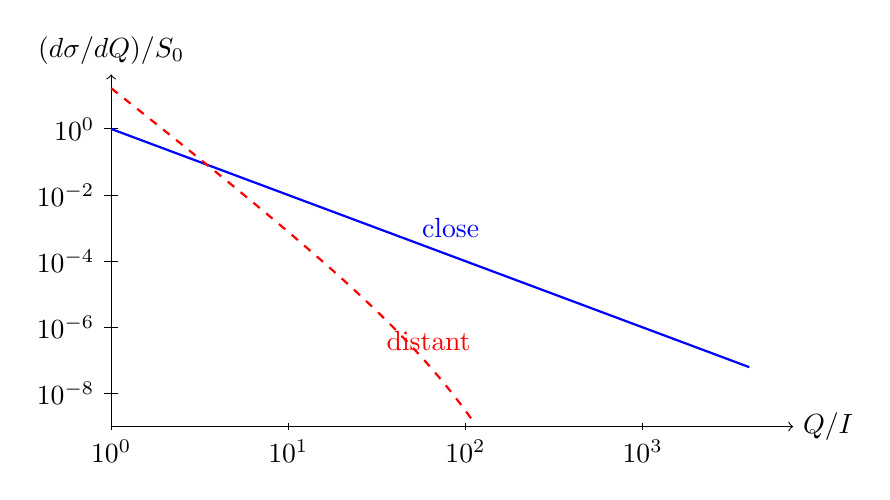
\begin{tikzpicture}[x=2.25cm,y=0.42cm]
\draw[->] (0,-9)--(3.85,-9) node[right] {$Q/I$};\draw[->] (0,-9)--(0,1.65) node[above] {$(d\sigma/dQ)/S_0$};
\draw (0,-8.9)--(0,-9.1) node[below] {$10^{0}$};
\draw (1,-8.9)--(1,-9.1) node[below] {$10^{1}$};
\draw (2,-8.9)--(2,-9.1) node[below] {$10^{2}$};
\draw (3,-8.9)--(3,-9.1) node[below] {$10^{3}$};
\draw (0.04,-8)--(-0.04,-8) node[left] {$10^{-8}$};
\draw (0.04,-6)--(-0.04,-6) node[left] {$10^{-6}$};
\draw (0.04,-4)--(-0.04,-4) node[left] {$10^{-4}$};
\draw (0.04,-2)--(-0.04,-2) node[left] {$10^{-2}$};
\draw (0.04,0)--(-0.04,0) node[left] {$10^{0}$};
\draw[blue,thick] plot coordinates {(0,0) (0.0112917,-0.0225834) (0.0225834,-0.0451669) (0.0338752,-0.0677503) (0.0451669,-0.0903338) (0.0564586,-0.112917) (0.0677503,-0.135501) (0.0790421,-0.158084) (0.0903338,-0.180668) (0.101626,-0.203251) (0.112917,-0.225834) (0.124209,-0.248418) (0.135501,-0.271001) (0.146792,-0.293585) (0.158084,-0.316168) (0.169376,-0.338752) (0.180668,-0.361335) (0.191959,-0.383919) (0.203251,-0.406502) (0.214543,-0.429086) (0.225834,-0.451669) (0.237126,-0.474252) (0.248418,-0.496836) (0.25971,-0.519419) (0.271001,-0.542003) (0.282293,-0.564586) (0.293585,-0.58717) (0.304877,-0.609753) (0.316168,-0.632337) (0.32746,-0.65492) (0.338752,-0.677503) (0.350043,-0.700087) (0.361335,-0.72267) (0.372627,-0.745254) (0.383919,-0.767837) (0.39521,-0.790421) (0.406502,-0.813004) (0.417794,-0.835588) (0.429086,-0.858171) (0.440377,-0.880754) (0.451669,-0.903338) (0.462961,-0.925921) (0.474252,-0.948505) (0.485544,-0.971088) (0.496836,-0.993672) (0.508128,-1.01626) (0.519419,-1.03884) (0.530711,-1.06142) (0.542003,-1.08401) (0.553294,-1.10659) (0.564586,-1.12917) (0.575878,-1.15176) (0.58717,-1.17434) (0.598461,-1.19692) (0.609753,-1.21951) (0.621045,-1.24209) (0.632337,-1.26467) (0.643628,-1.28726) (0.65492,-1.30984) (0.666212,-1.33242) (0.677503,-1.35501) (0.688795,-1.37759) (0.700087,-1.40017) (0.711379,-1.42276) (0.72267,-1.44534) (0.733962,-1.46792) (0.745254,-1.49051) (0.756546,-1.51309) (0.767837,-1.53567) (0.779129,-1.55826) (0.790421,-1.58084) (0.801712,-1.60342) (0.813004,-1.62601) (0.824296,-1.64859) (0.835588,-1.67118) (0.846879,-1.69376) (0.858171,-1.71634) (0.869463,-1.73893) (0.880754,-1.76151) (0.892046,-1.78409) (0.903338,-1.80668) (0.91463,-1.82926) (0.925921,-1.85184) (0.937213,-1.87443) (0.948505,-1.89701) (0.959797,-1.91959) (0.971088,-1.94218) (0.98238,-1.96476) (0.993672,-1.98734) (1.00496,-2.00993) (1.01626,-2.03251) (1.02755,-2.05509) (1.03884,-2.07768) (1.05013,-2.10026) (1.06142,-2.12284) (1.07271,-2.14543) (1.08401,-2.16801) (1.0953,-2.19059) (1.10659,-2.21318) (1.11788,-2.23576) (1.12917,-2.25834) (1.14046,-2.28093) (1.15176,-2.30351) (1.16305,-2.3261) (1.17434,-2.34868) (1.18563,-2.37126) (1.19692,-2.39385) (1.20821,-2.41643) (1.21951,-2.43901) (1.2308,-2.4616) (1.24209,-2.48418) (1.25338,-2.50676) (1.26467,-2.52935) (1.27596,-2.55193) (1.28726,-2.57451) (1.29855,-2.5971) (1.30984,-2.61968) (1.32113,-2.64226) (1.33242,-2.66485) (1.34372,-2.68743) (1.35501,-2.71001) (1.3663,-2.7326) (1.37759,-2.75518) (1.38888,-2.77776) (1.40017,-2.80035) (1.41147,-2.82293) (1.42276,-2.84551) (1.43405,-2.8681) (1.44534,-2.89068) (1.45663,-2.91326) (1.46792,-2.93585) (1.47922,-2.95843) (1.49051,-2.98102) (1.5018,-3.0036) (1.51309,-3.02618) (1.52438,-3.04877) (1.53567,-3.07135) (1.54697,-3.09393) (1.55826,-3.11652) (1.56955,-3.1391) (1.58084,-3.16168) (1.59213,-3.18427) (1.60342,-3.20685) (1.61472,-3.22943) (1.62601,-3.25202) (1.6373,-3.2746) (1.64859,-3.29718) (1.65988,-3.31977) (1.67118,-3.34235) (1.68247,-3.36493) (1.69376,-3.38752) (1.70505,-3.4101) (1.71634,-3.43268) (1.72763,-3.45527) (1.73893,-3.47785) (1.75022,-3.50043) (1.76151,-3.52302) (1.7728,-3.5456) (1.78409,-3.56818) (1.79538,-3.59077) (1.80668,-3.61335) (1.81797,-3.63594) (1.82926,-3.65852) (1.84055,-3.6811) (1.85184,-3.70369) (1.86313,-3.72627) (1.87443,-3.74885) (1.88572,-3.77144) (1.89701,-3.79402) (1.9083,-3.8166) (1.91959,-3.83919) (1.93088,-3.86177) (1.94218,-3.88435) (1.95347,-3.90694) (1.96476,-3.92952) (1.97605,-3.9521) (1.98734,-3.97469) (1.99864,-3.99727) (2.00993,-4.01985) (2.02122,-4.04244) (2.03251,-4.06502) (2.0438,-4.0876) (2.05509,-4.11019) (2.06639,-4.13277) (2.07768,-4.15535) (2.08897,-4.17794) (2.10026,-4.20052) (2.11155,-4.2231) (2.12284,-4.24569) (2.13414,-4.26827) (2.14543,-4.29086) (2.15672,-4.31344) (2.16801,-4.33602) (2.1793,-4.35861) (2.19059,-4.38119) (2.20189,-4.40377) (2.21318,-4.42636) (2.22447,-4.44894) (2.23576,-4.47152) (2.24705,-4.49411) (2.25834,-4.51669) (2.26964,-4.53927) (2.28093,-4.56186) (2.29222,-4.58444) (2.30351,-4.60702) (2.3148,-4.62961) (2.3261,-4.65219) (2.33739,-4.67477) (2.34868,-4.69736) (2.35997,-4.71994) (2.37126,-4.74252) (2.38255,-4.76511) (2.39385,-4.78769) (2.40514,-4.81027) (2.41643,-4.83286) (2.42772,-4.85544) (2.43901,-4.87802) (2.4503,-4.90061) (2.4616,-4.92319) (2.47289,-4.94578) (2.48418,-4.96836) (2.49547,-4.99094) (2.50676,-5.01353) (2.51805,-5.03611) (2.52935,-5.05869) (2.54064,-5.08128) (2.55193,-5.10386) (2.56322,-5.12644) (2.57451,-5.14903) (2.5858,-5.17161) (2.5971,-5.19419) (2.60839,-5.21678) (2.61968,-5.23936) (2.63097,-5.26194) (2.64226,-5.28453) (2.65356,-5.30711) (2.66485,-5.32969) (2.67614,-5.35228) (2.68743,-5.37486) (2.69872,-5.39744) (2.71001,-5.42003) (2.72131,-5.44261) (2.7326,-5.46519) (2.74389,-5.48778) (2.75518,-5.51036) (2.76647,-5.53294) (2.77776,-5.55553) (2.78906,-5.57811) (2.80035,-5.6007) (2.81164,-5.62328) (2.82293,-5.64586) (2.83422,-5.66845) (2.84551,-5.69103) (2.85681,-5.71361) (2.8681,-5.7362) (2.87939,-5.75878) (2.89068,-5.78136) (2.90197,-5.80395) (2.91326,-5.82653) (2.92456,-5.84911) (2.93585,-5.8717) (2.94714,-5.89428) (2.95843,-5.91686) (2.96972,-5.93945) (2.98102,-5.96203) (2.99231,-5.98461) (3.0036,-6.0072) (3.01489,-6.02978) (3.02618,-6.05236) (3.03747,-6.07495) (3.04877,-6.09753) (3.06006,-6.12011) (3.07135,-6.1427) (3.08264,-6.16528) (3.09393,-6.18786) (3.10522,-6.21045) (3.11652,-6.23303) (3.12781,-6.25562) (3.1391,-6.2782) (3.15039,-6.30078) (3.16168,-6.32337) (3.17297,-6.34595) (3.18427,-6.36853) (3.19556,-6.39112) (3.20685,-6.4137) (3.21814,-6.43628) (3.22943,-6.45887) (3.24072,-6.48145) (3.25202,-6.50403) (3.26331,-6.52662) (3.2746,-6.5492) (3.28589,-6.57178) (3.29718,-6.59437) (3.30848,-6.61695) (3.31977,-6.63953) (3.33106,-6.66212) (3.34235,-6.6847) (3.35364,-6.70728) (3.36493,-6.72987) (3.37623,-6.75245) (3.38752,-6.77503) (3.39881,-6.79762) (3.4101,-6.8202) (3.42139,-6.84278) (3.43268,-6.86537) (3.44398,-6.88795) (3.45527,-6.91054) (3.46656,-6.93312) (3.47785,-6.9557) (3.48914,-6.97829) (3.50043,-7.00087) (3.51173,-7.02345) (3.52302,-7.04604) (3.53431,-7.06862) (3.5456,-7.0912) (3.55689,-7.11379) (3.56818,-7.13637) (3.57948,-7.15895) (3.59077,-7.18154) (3.60206,-7.20412)};
\draw[red,thick,dashed] plot coordinates {(0,1.23155) (0.0112917,1.18371) (0.0225834,1.13586) (0.0338752,1.08799) (0.0451669,1.04011) (0.0564586,0.992204) (0.0677503,0.944283) (0.0790421,0.896344) (0.0903338,0.848387) (0.101626,0.800412) (0.112917,0.752417) (0.124209,0.704404) (0.135501,0.656372) (0.146792,0.608319) (0.158084,0.560247) (0.169376,0.512155) (0.180668,0.464043) (0.191959,0.415909) (0.203251,0.367755) (0.214543,0.319579) (0.225834,0.271382) (0.237126,0.223162) (0.248418,0.17492) (0.25971,0.126656) (0.271001,0.0783679) (0.282293,0.0300568) (0.293585,-0.0182781) (0.304877,-0.0666372) (0.316168,-0.115021) (0.32746,-0.16343) (0.338752,-0.211864) (0.350043,-0.260323) (0.361335,-0.30881) (0.372627,-0.357322) (0.383919,-0.405862) (0.39521,-0.45443) (0.406502,-0.503026) (0.417794,-0.55165) (0.429086,-0.600303) (0.440377,-0.648986) (0.451669,-0.697699) (0.462961,-0.746443) (0.474252,-0.795217) (0.485544,-0.844024) (0.496836,-0.892863) (0.508128,-0.941735) (0.519419,-0.990641) (0.530711,-1.03958) (0.542003,-1.08856) (0.553294,-1.13757) (0.564586,-1.18661) (0.575878,-1.2357) (0.58717,-1.28482) (0.598461,-1.33398) (0.609753,-1.38317) (0.621045,-1.43241) (0.632337,-1.48169) (0.643628,-1.53101) (0.65492,-1.58038) (0.666212,-1.62978) (0.677503,-1.67923) (0.688795,-1.72873) (0.700087,-1.77827) (0.711379,-1.82786) (0.72267,-1.8775) (0.733962,-1.92718) (0.745254,-1.97692) (0.756546,-2.02671) (0.767837,-2.07655) (0.779129,-2.12644) (0.790421,-2.17639) (0.801712,-2.2264) (0.813004,-2.27646) (0.824296,-2.32658) (0.835588,-2.37676) (0.846879,-2.427) (0.858171,-2.4773) (0.869463,-2.52767) (0.880754,-2.57811) (0.892046,-2.62861) (0.903338,-2.67918) (0.91463,-2.72982) (0.925921,-2.78053) (0.937213,-2.83131) (0.948505,-2.88218) (0.959797,-2.93311) (0.971088,-2.98413) (0.98238,-3.03523) (0.993672,-3.08642) (1.00496,-3.13768) (1.01626,-3.18904) (1.02755,-3.24048) (1.03884,-3.29202) (1.05013,-3.34365) (1.06142,-3.39538) (1.07271,-3.44721) (1.08401,-3.49913) (1.0953,-3.55117) (1.10659,-3.6033) (1.11788,-3.65555) (1.12917,-3.70791) (1.14046,-3.76039) (1.15176,-3.81298) (1.16305,-3.8657) (1.17434,-3.91854) (1.18563,-3.97151) (1.19692,-4.02461) (1.20821,-4.07784) (1.21951,-4.13121) (1.2308,-4.18473) (1.24209,-4.23838) (1.25338,-4.29219) (1.26467,-4.34615) (1.27596,-4.40027) (1.28726,-4.45456) (1.29855,-4.509) (1.30984,-4.56362) (1.32113,-4.61841) (1.33242,-4.67339) (1.34372,-4.72854) (1.35501,-4.78389) (1.3663,-4.83944) (1.37759,-4.89518) (1.38888,-4.95113) (1.40017,-5.00729) (1.41147,-5.06366) (1.42276,-5.12026) (1.43405,-5.17709) (1.44534,-5.23416) (1.45663,-5.29146) (1.46792,-5.34902) (1.47922,-5.40683) (1.49051,-5.4649) (1.5018,-5.52324) (1.51309,-5.58186) (1.52438,-5.64076) (1.53567,-5.69995) (1.54697,-5.75945) (1.55826,-5.81925) (1.56955,-5.87937) (1.58084,-5.93982) (1.59213,-6.0006) (1.60342,-6.06172) (1.61472,-6.1232) (1.62601,-6.18504) (1.6373,-6.24726) (1.64859,-6.30985) (1.65988,-6.37284) (1.67118,-6.43624) (1.68247,-6.50005) (1.69376,-6.56429) (1.70505,-6.62896) (1.71634,-6.69409) (1.72763,-6.75968) (1.73893,-6.82575) (1.75022,-6.8923) (1.76151,-6.95936) (1.7728,-7.02694) (1.78409,-7.09504) (1.79538,-7.16369) (1.80668,-7.2329) (1.81797,-7.30268) (1.82926,-7.37306) (1.84055,-7.44404) (1.85184,-7.51564) (1.86313,-7.58789) (1.87443,-7.66079) (1.88572,-7.73437) (1.89701,-7.80864) (1.9083,-7.88363) (1.91959,-7.95934) (1.93088,-8.03582) (1.94218,-8.11306) (1.95347,-8.19109) (1.96476,-8.26995) (1.97605,-8.34964) (1.98734,-8.43018) (1.99864,-8.51162) (2.00993,-8.59396) (2.02122,-8.67723) (2.03251,-8.76145) (2.0438,-8.84666) (2.05509,-8.93288)};
\node[blue,right] at (1.7,-3) {close};\node[red,right] at (1.5,-6.4) {distant};
\end{tikzpicture}
\end{center}
The close curve is shown up to its heavy-projectile endpoint
$Y=4S=4000$.  For finite $M$ replace it by
$Y=4000[M/(M+m)]^2$.  The distant curve falls exponentially when
$Q\gtrsim\hbar v/d$, in addition to its initial $Q^{-4}$ dependence.

\medskip\noindent\textbf{(b)} Divide collision numbers by $S_0I$
and energy transfers by $S_0I^2$.  For close collisions,
\[
n_c=\int_1^Yy^{-2}dy=1-Y^{-1},\qquad
\ell_c=\int_1^Yy^{-1}dy=\ln Y.
\]
For the distant spectrum the exact model integrals are
\[
n_d=4\int_1^\infty y^{-4}B(y/2\sqrt S)dy,\qquad
\ell_d=4\int_1^\infty y^{-3}B(y/2\sqrt S)dy.
\]
To expose the physics, use the low-$x$ expansion
$B(x)=\ln(2/x)-\gamma_E+O(x^2\ln^2x)$ in the nonrelativistic limit.
Write $L_0=\ln(4\sqrt S)-\gamma_E$.  Then
\begin{align*}
n_d&\simeq4\int_1^\infty y^{-4}(L_0-\ln y)dy
 =\frac43(L_0-\tfrac13),\\
\ell_d&\simeq4\int_1^\infty y^{-3}(L_0-\ln y)dy
 =2(L_0-\tfrac12).
\end{align*}
Here $\int_1^\infty y^{-p}dy=(p-1)^{-1}$ and differentiating it
with respect to $p$ gives the logarithmic integral
$(p-1)^{-2}$.  The tail beyond the virtual-photon cutoff changes
only small corrections for $S\gg1$.  At $S=1000$, direct Bessel
quadrature gives the values in the supplementary calculation;
rounded to the accuracy of the model,
\[
n_c=0.99975,\quad n_d=5.23393,\qquad
\ell_c=8.29405,\quad\ell_d=7.51412.
\]
Thus distant events are about five times more numerous, and their
mean transfer $I\ell_d/n_d\simeq1.44I$ is much smaller than the
close mean $I\ell_c/n_c\simeq8.30I$.  Their energy losses are
nevertheless comparable, about $48\%$ and $52\%$ of the sum.

For a number density $N_a$ of these one-electron atoms, the leading
nonrelativistic heavy-projectile stopping power is
\begin{align*}
-\frac{dE}{dx}
&=N_aS_0I^2(\ell_c+\ell_d)\\
&\simeq\frac{2\pi N_az^2e^4}{mv^2}
 [\ln(64S^2)-2\gamma_E-1]\\
&=\frac{4\pi N_az^2e^4}{mv^2}
 \ln\frac{2mv^2}{I_{\rm eff}},
\qquad
I_{\rm eff}=\frac12 e^{\gamma_E+1/2}I\simeq1.47I.
\end{align*}
This is Bethe's logarithmic form (13.14), with an effective mean
excitation energy of the order of the ionization energy.  The
photoabsorption model omits discrete excitation lines and uses a
crude separation of close and distant events, so it cannot fix the
exact atomic mean-excitation constant.  If one simply sets that
constant to $I$, Bethe's dimensionless sum is
$2\ln(4S)=16.5881$, versus approximately $15.8082$ here, a difference
of less than $5\%$ at the stipulated speed.  For finite projectile
mass the recoil factor in $Y$ reduces the close contribution in the
way already shown.

\Needspace{5\baselineskip}
\par\bigskip
\noindent\textbf{15.13}\quad In the decay of a pi meson at rest a mu meson and a neutrino are created. The total kinetic energy available is $(m_{\pi}-m_{\mu})c^{2}=34$ MeV. The mu meson has a kinetic energy of 4.1 MeV. Determine the number of quanta emitted per unit energy interval because of the sudden creation of the moving mu meson. Assuming that the photons are emitted perpendicular to the direction of motion of the mu meson (actually it is a $\sin^{2}\theta$ distribution), show that the maximum photon energy is 17 MeV. Find how many quanta are emitted with energies greater than one-tenth of the maximum, and compare your result with the observed ratio of radiative pi-mu decays. [$1.24\pm0.25\times10^{-4}$ for muons with kinetic energy less than 3.4 MeV. See also H.~Primakoff, \emph{Phys. Rev.}, \textbf{84}, 1255 (1951).]
\solution

Let $\varepsilon=\hbar\omega$ and neglect radiation from the
stationary parent pion and the neutral neutrino.  For a suddenly
created muon with speed $c\beta$, (15.65) gives
\[
\frac{d^2N}{d\varepsilon\,d\Omega}
=\frac{\alpha}{4\pi^2\varepsilon}
 \frac{\beta^2\sin^2\theta}{(1-\beta\cos\theta)^2}.
\]
Put $x=\cos\theta$.  The same elementary substitution
$y=1-\beta x$ as in Problem 15.3 gives
\[
\int_{-1}^{1}\frac{\beta^2(1-x^2)}{(1-\beta x)^2}dx
=\frac2\beta\ln\frac{1+\beta}{1-\beta}-4.
\]
Therefore
\[
\boxed{\frac{dN}{d\varepsilon}=\frac{C(\beta)}\varepsilon,
\qquad C(\beta)=\frac{\alpha}{\pi}
\left[\frac1\beta\ln\frac{1+\beta}{1-\beta}-2\right].}
\]
For $m_\mu c^2=105.66$ MeV and $T_\mu=4.1$ MeV,
$\beta=\sqrt{T_\mu(T_\mu+2m_\mu c^2)}/(T_\mu+m_\mu c^2)
=0.270764$ and $C=1.18800\times10^{-4}$.
The nonrelativistic limit is $C\simeq2\alpha\beta^2/(3\pi)$.

To implement the stipulated perpendicular-photon approximation, use
$c=1$ temporarily, let $\Delta=m_\pi-m_\mu=34$ MeV, and call the
muon momentum $p$.  The neutrino momentum is then
$\sqrt{p^2+\varepsilon^2}$, so energy conservation reads
\[
\Delta=T_\mu+\varepsilon+\sqrt{T_\mu^2+2m_\mu T_\mu+\varepsilon^2}.
\]
Squaring and cancelling the common $T_\mu^2$ and $\varepsilon^2$
terms gives
\[
\boxed{T_\mu(\varepsilon)
=\frac{\Delta(\Delta-2\varepsilon)}{2(m_\pi-\varepsilon)},
\qquad 0\leq\varepsilon\leq\Delta/2=17\ {\rm MeV}.}
\]
The maximum occurs at vanishing muon momentum.  With the stated
rounded masses the zero-photon energy from this relation is
$4.139$ MeV, consistent with the quoted $4.1$ MeV accuracy.
A frozen soft coefficient gives the requested count
\[
\boxed{N(\varepsilon>1.7\ {\rm MeV})
\simeq C\ln(17/1.7)=2.7355\times10^{-4}.}
\]
This is about $2.2$ times the measured ratio.  There are two distinct
limitations to that direct comparison.  First, emission of an
energetic photon reduces the muon speed, so the constant soft
coefficient overestimates the high-energy portion.  As a simple
kinematic improvement, insert the $\beta[T_\mu(\varepsilon)]$
just derived into $C$ and integrate:
\[
\int_{1.7}^{17}\frac{C(\beta[T_\mu(\varepsilon)])}{\varepsilon}
 d\varepsilon=1.7495\times10^{-4}.
\]
Second, the experimental cut $T_\mu<3.4$ MeV does not correspond
to $\varepsilon>1.7$ MeV.  In this same perpendicular model it is
\[
\varepsilon>\frac{\Delta^2-2(3.4)m_\pi}{2(\Delta-3.4)}
=3.3711\ {\rm MeV}.
\]
With this matched cut the improved estimate is
$1.0329\times10^{-4}$, comparable to
$(1.24\pm0.25)\times10^{-4}$.  This last agreement is at the level
of the model: the real angular distribution, decay phase space and
non-soft amplitude are not replaced exactly by perpendicular emission
and a velocity-dependent soft coefficient.


\Needspace{5\baselineskip}
\par\bigskip
\noindent\textbf{15.14}\quad In internal conversion, the nucleus makes a transition from one state to another and an orbital electron is ejected. The electron has a kinetic energy equal to the transition energy minus its binding energy. For a conversion line of 1 MeV determine the number of quanta emitted per unit energy because of the sudden ejection of the electron. What fraction of the electrons will have energies less than 99\% of the total energy? Will this low-energy tail on the conversion line be experimentally observable?
\solution

Interpret the 1 MeV conversion line as the electron's kinetic energy
$T_0$, as specified in the question.  Initially bound electronic
motion, nuclear recoil and atomic relaxation are neglected in the
sudden-ejection approximation.  Then
\[
\gamma=1+\frac{T_0}{m_ec^2}=2.956951,
\qquad \beta=\sqrt{1-\gamma^{-2}}=0.941079.
\]
The single-charge endpoint formula (15.67), or the angular integral
in Problem 15.13, gives
\[
\boxed{\frac{dN}{d\varepsilon}
=\frac{\alpha}{\pi\varepsilon}
\left[\frac1\beta\ln\frac{1+\beta}{1-\beta}-2\right]
=\frac{0.00398042}{\varepsilon}.}
\]
If $\varepsilon$ is measured in MeV, the displayed density is per
MeV.  The spectrum has this form for soft photons; the electron's
kinetic-energy budget bounds its endpoint by $\varepsilon\leq1$ MeV.

An electron below $0.99T_0$ has lost more than $0.01T_0=10$ keV.
At leading order in the emission probability, the requested fraction
is the one-photon number on this band:
\[
\boxed{f\simeq0.00398042\int_{0.01}^{1}\frac{d\varepsilon}{\varepsilon}
=0.00398042\ln100=0.01833,}
\]
about $1.8\%$.  Multiple-photon corrections are higher order in
this small probability.  Using the full relativistic electron energy
$E_0=T_0+m_ec^2$ in the phrase ``99\% of the total energy'' instead
would impose $\varepsilon>0.01E_0=15.11$ keV and give $f=0.01669$;
the usual line-energy convention refers to the measured kinetic
energy and gives the first value.

This is an intrinsically observable, percent-level continuum below
the conversion peak: a measurement resolving 10 keV and collecting
adequate counts can distinguish such a tail.  No detector resolution
or background is specified, so its visibility in any particular
apparatus cannot be asserted.  External bremsstrahlung and electron
energy loss in the source also make low-energy tails and must be
controlled to isolate this intrinsic contribution.  The estimated
fraction is only logarithmically sensitive to the endpoint, but
holding $\beta$ fixed all the way to 1 MeV is still an extrapolation
of the soft spectrum, not an exact conversion-line shape.


\Needspace{5\baselineskip}
\par\bigskip
\noindent\textbf{15.15}\quad One of the decay modes of a $\mathrm{K}^{+}$ meson is the three-pion decay, $\mathrm{K}^{+}\to\pi^{+}\pi^{+}\pi^{-}$. The energy release is 75 MeV, small enough that the pions can be treated nonrelativistically in rough approximation.
\begin{enumerate}
\item[(a)] Show that the differential spectrum of radiated intensity at low frequencies in the K meson rest frame is approximately
\[
\frac{d^{2}I}{d\omega\;d\Omega}\simeq\frac{2e^{2}}{\pi^{2}c}\cdot\frac{T_{-}}{m_{\pi}c^{2}}\cdot\sin^{2}\theta
\]
where $T_{-}$ is the kinetic energy of the negative pion and $\theta$ is the angle of emission of the photon relative to the momentum of the negative pion.
\item[(b)] Estimate the branching ratio for emission of a photon of energy greater than $\Delta$ relative to the nonradiative three-pion decay. What is its numerical value for $\Delta=1$ MeV? 10 MeV? Compare with experiment ($\sim2\times10^{-3}$ for $\Delta=11$ MeV).
\end{enumerate}
\solution

\medskip\noindent\textbf{(a)} In the kaon rest frame momentum
conservation, to leading nonrelativistic order for equal pion masses,
is
\[
\mathbf v_{+1}+\mathbf v_{+2}+\mathbf v_-=0.
\]
The parent's initial velocity is zero.  The electric-dipole endpoint
amplitude of the three created pions is consequently
\[
\mathbf J=\frac ecP(\mathbf v_{+1}+\mathbf v_{+2}-\mathbf v_-)
=-\frac{2e}{c}P\mathbf v_-.
\]
Using $v_-^2=2T_-/m_\pi$ in $|\mathbf J|^2/(4\pi^2c)$ gives
\[
\boxed{\frac{d^2I}{d\omega\,d\Omega}
=\frac{2e^2}{\pi^2c}\frac{T_-}{m_\pi c^2}\sin^2\theta.}
\]
The direction is measured from the negative pion because its velocity
alone expresses the charge-weighted total after using momentum
conservation.  Integrating $\sin^2\theta$ yields
\[
\frac{dN}{d\varepsilon}
=\frac{16\alpha}{3\pi}\frac{T_-}{m_\pi c^2}
 \frac1\varepsilon.
\]

\medskip\noindent\textbf{(b)} The nonradiative Dalitz distribution
is not specified, so a numerical branching ratio requires an
assumption about its average $T_-$.  For a constant decay amplitude
and the symmetric nonrelativistic three-body phase space, all three
pions have the same mean energy, $\langle T_-\rangle=Q/3=25$ MeV,
where $Q=75$ MeV.  This also follows by permutation symmetry from
$\sum T_i=Q$.  With $m_\pi c^2=139.6$ MeV,
\[
C_3=\frac{16\alpha}{3\pi}\frac{25}{139.6}=0.00221855.
\]
Extrapolating a frozen soft coefficient up to the available energy
gives $B_0(\Delta)=C_3\ln(Q/\Delta)$.
A more useful rough estimate accounts for the reduced kinetic
budget by $\langle T_-(\varepsilon)\rangle\simeq(Q-\varepsilon)/3$.
It gives the elementary integral
\begin{align*}
B(\Delta)&\simeq C_3\int_\Delta^Q
 \left(1-\frac{\varepsilon}{Q}\right)\frac{d\varepsilon}{\varepsilon}\\
&=\boxed{C_3\left[\ln\frac Q\Delta-1+\frac\Delta Q\right].}
\end{align*}
Here $B$ is relative to nonradiative three-pion decay, as requested.
The resulting estimates are
\begin{center}
\begin{tabular}{rrr}
\toprule
$\Delta$ (MeV)&Frozen soft $B_0$&Reduced-budget $B$\\
\midrule
1&$9.579\times10^{-3}$&$7.390\times10^{-3}$\\
10&$4.470\times10^{-3}$&$2.547\times10^{-3}$\\
11&$4.259\times10^{-3}$&$2.366\times10^{-3}$\\
\bottomrule
\end{tabular}
\end{center}
The last improved value is close in scale to the stated
$2\times10^{-3}$ measurement.  It is not a precision prediction:
the available three-pion phase space and the actual decay amplitude
also change when a photon is emitted.  Even the exact endpoint is
$[M_K^2-9m_\pi^2]c^2/(2M_K)\simeq69.3$ MeV rather than $Q$,
because the pion system recoils; $Q$ is its nonrelativistic
approximation.  The coefficient of the soft logarithm follows from
part (a), while the nonlogarithmic correction and hard-photon tail
depend on the additional decay model.  The table states explicitly
which approximation supplies those estimates.


\Needspace{5\baselineskip}
\par\bigskip
\noindent\textbf{15.16}\quad One of the decay modes of the charged K meson ($M_{\mathrm{K}}=493.7$ MeV) is $\mathrm{K}^{+}\to\pi^{+}\pi^{0}$ ($M_{\pi^{+}}=139.6$ MeV, $M_{\pi^{0}}=135.0$ MeV). Inner bremsstrahlung is emitted by the creation of the positive pion. A study of this radiative decay mode was made by Edwards et al.\ [\emph{Phys. Rev.} \textbf{D5}, 2720 (1972)].
\begin{enumerate}
\item[(a)] Calculate the classical distribution in angle and frequency of soft photons and compare with the data of Fig.~6 of Edwards et al. Compute the classical distribution also for $\beta=0.71$, corresponding to a charged pion of kinetic energy 58 MeV, and compare.
\item[(b)] Estimate the number of radiative decays for charged pion kinetic energies on the interval, $55\ \mathrm{MeV}\leq T_{\pi}\leq90\ \mathrm{MeV}$, as a fraction of \emph{all} $\mathrm{K}^{+}$ decays (the $\pi^{+}\pi^{0}$ decay mode is 21\% of all decays). You can treat the kinematics, including the photon, correctly, or you can approximate reality with an idealization that has the neutral pion always with the same momentum and the photon and the charged pion with parallel momenta (see part a for justification of this assumption). This idealization permits you to correlate directly the limits on the charged pion's kinetic energy with that of the photon. \erratum{At fixed neutral momentum equal to its nonradiative value, this shortcut cannot also conserve energy exactly for a nonzero photon. Use it only as a momentum-based estimate, or use the full kinematics.} Compare your estimate with the experimental value for the branching ratio for $\pi^{+}\pi^{0}\gamma$ (with the limited range of $\pi^{+}$ energies) of $(2.75\pm0.15)\times10^{-4}$.
\end{enumerate}
\solution

\medskip\noindent\textbf{(a)} Use $c=1$ for the kinematics, with all
masses in MeV.  Two-body energy and momentum conservation give
\[
E_* =\frac{M_K^2+m_+^2-m_0^2}{2M_K}=248.129279\ {\rm MeV},
\quad p_* =\sqrt{E_*^2-m_+^2}=205.134051\ {\rm MeV},
\]
\[
T_*=108.529279\ {\rm MeV},\qquad \beta_*=p_*/E_*=0.82672247.
\]
The initial kaon is stationary and the neutral pion has no charge.
The soft radiation is therefore the endpoint radiation of the charged
pion alone.  Restoring $c$ in the spectral intensity gives
\[
\boxed{\frac{d^2I}{d\omega\,d\Omega}
=\frac{e^2}{4\pi^2c}\frac{\beta^2\sin^2\theta}
 {(1-\beta\cos\theta)^2},\qquad
\frac{d^2N}{d\varepsilon\,dx}
=\frac{\alpha}{2\pi\varepsilon}
 \frac{\beta^2(1-x^2)}{(1-\beta x)^2},\quad x=\cos\theta.}
\]
The intensity is independent of frequency in the soft limit, while
the photon number is proportional to $1/\varepsilon$.  Differentiating
$(1-x^2)/(1-\beta x)^2$ gives
$2(\beta-x)/(1-\beta x)^3$, so its maximum is at
$x=\beta$: $\theta_{\max}=34.24^\circ$ for $\beta_*$ and
$44.77^\circ$ for $\beta=0.71$.

Figure 6 was checked in Edwards et al.'s original preprint,
COO-1195-230 (December 1971), Fig.~6, p.~26 of the OSTI scan.
It has 24 events in six equal $x$ bins and imposes
$58\leq T_\pi\leq90$ MeV.  Normalizing either classical curve to
24 events gives the comparison
\begin{center}
\begin{tabular}{lrrrrrr}
\toprule
$x$ bin&$[-1,-2/3]$&$[-2/3,-1/3]$&$[-1/3,0]$&$[0,1/3]$&$[1/3,2/3]$&$[2/3,1]$\\
\midrule
Observed&0&1&3&5&9&6\\
$\beta=0.82672$&0.35&1.22&2.44&4.25&7.07&8.66\\
$\beta=0.71$&0.50&1.66&3.16&5.07&7.24&6.38\\
\bottomrule
\end{tabular}
\end{center}
\begin{center}% Generated by supplementary/check_ch15.py
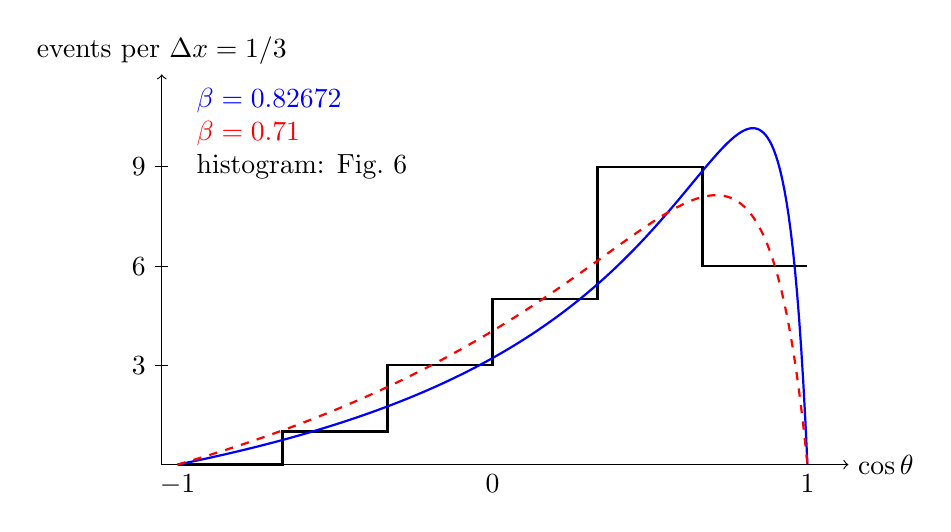
\begin{tikzpicture}[x=4cm,y=0.42cm]
\draw[->] (-1.05,0)--(1.13,0) node[right] {$\cos\theta$};\draw[->] (-1.05,0)--(-1.05,11.8) node[above] {events per $\Delta x=1/3$};
\node[below] at (-1,0) {$ -1 $};
\node[below] at (0,0) {$ 0 $};
\node[below] at (1,0) {$ 1 $};
\draw (-1.03,3)--(-1.07,3) node[left] {$ 3 $};
\draw (-1.03,6)--(-1.07,6) node[left] {$ 6 $};
\draw (-1.03,9)--(-1.07,9) node[left] {$ 9 $};
\draw[black,thick] plot coordinates {(-1,0) (-0.666667,0) (-0.666667,1) (-0.333333,1) (-0.333333,3) (0,3) (0,5) (0.333333,5) (0.333333,9) (0.666667,9) (0.666667,6) (1,6)};
\draw[blue,thick] plot coordinates {(-1,0) (-0.993333,0.0129005) (-0.986667,0.0258711) (-0.98,0.0389124) (-0.973333,0.0520248) (-0.966667,0.065209) (-0.96,0.0784655) (-0.953333,0.091795) (-0.946667,0.105198) (-0.94,0.118675) (-0.933333,0.132227) (-0.926667,0.145854) (-0.92,0.159557) (-0.913333,0.173337) (-0.906667,0.187194) (-0.9,0.201129) (-0.893333,0.215143) (-0.886667,0.229235) (-0.88,0.243408) (-0.873333,0.257661) (-0.866667,0.271995) (-0.86,0.286411) (-0.853333,0.30091) (-0.846667,0.315492) (-0.84,0.330158) (-0.833333,0.344908) (-0.826667,0.359744) (-0.82,0.374667) (-0.813333,0.389676) (-0.806667,0.404772) (-0.8,0.419957) (-0.793333,0.435232) (-0.786667,0.450596) (-0.78,0.466051) (-0.773333,0.481597) (-0.766667,0.497236) (-0.76,0.512968) (-0.753333,0.528793) (-0.746667,0.544714) (-0.74,0.56073) (-0.733333,0.576842) (-0.726667,0.593052) (-0.72,0.60936) (-0.713333,0.625767) (-0.706667,0.642274) (-0.7,0.658882) (-0.693333,0.675591) (-0.686667,0.692403) (-0.68,0.709319) (-0.673333,0.726339) (-0.666667,0.743465) (-0.66,0.760697) (-0.653333,0.778037) (-0.646667,0.795485) (-0.64,0.813042) (-0.633333,0.83071) (-0.626667,0.848489) (-0.62,0.86638) (-0.613333,0.884385) (-0.606667,0.902505) (-0.6,0.92074) (-0.593333,0.939092) (-0.586667,0.957562) (-0.58,0.97615) (-0.573333,0.994859) (-0.566667,1.01369) (-0.56,1.03264) (-0.553333,1.05172) (-0.546667,1.07092) (-0.54,1.09024) (-0.533333,1.1097) (-0.526667,1.12928) (-0.52,1.14899) (-0.513333,1.16883) (-0.506667,1.1888) (-0.5,1.20891) (-0.493333,1.22915) (-0.486667,1.24953) (-0.48,1.27005) (-0.473333,1.2907) (-0.466667,1.31149) (-0.46,1.33243) (-0.453333,1.35351) (-0.446667,1.37473) (-0.44,1.3961) (-0.433333,1.41761) (-0.426667,1.43928) (-0.42,1.46109) (-0.413333,1.48305) (-0.406667,1.50517) (-0.4,1.52745) (-0.393333,1.54988) (-0.386667,1.57246) (-0.38,1.59521) (-0.373333,1.61812) (-0.366667,1.64119) (-0.36,1.66442) (-0.353333,1.68782) (-0.346667,1.71139) (-0.34,1.73513) (-0.333333,1.75904) (-0.326667,1.78312) (-0.32,1.80738) (-0.313333,1.83182) (-0.306667,1.85643) (-0.3,1.88122) (-0.293333,1.9062) (-0.286667,1.93136) (-0.28,1.95671) (-0.273333,1.98224) (-0.266667,2.00797) (-0.26,2.03389) (-0.253333,2.06) (-0.246667,2.08631) (-0.24,2.11282) (-0.233333,2.13952) (-0.226667,2.16644) (-0.22,2.19355) (-0.213333,2.22088) (-0.206667,2.24841) (-0.2,2.27616) (-0.193333,2.30412) (-0.186667,2.33229) (-0.18,2.36069) (-0.173333,2.38931) (-0.166667,2.41815) (-0.16,2.44722) (-0.153333,2.47652) (-0.146667,2.50604) (-0.14,2.53581) (-0.133333,2.56581) (-0.126667,2.59604) (-0.12,2.62653) (-0.113333,2.65725) (-0.106667,2.68823) (-0.1,2.71945) (-0.0933333,2.75093) (-0.0866667,2.78266) (-0.08,2.81465) (-0.0733333,2.84691) (-0.0666667,2.87943) (-0.06,2.91221) (-0.0533333,2.94527) (-0.0466667,2.9786) (-0.04,3.01221) (-0.0333333,3.0461) (-0.0266667,3.08028) (-0.02,3.11474) (-0.0133333,3.14949) (-0.00666667,3.18454) (0,3.21988) (0.00666667,3.25552) (0.0133333,3.29147) (0.02,3.32773) (0.0266667,3.36429) (0.0333333,3.40117) (0.04,3.43838) (0.0466667,3.4759) (0.0533333,3.51375) (0.06,3.55192) (0.0666667,3.59044) (0.0733333,3.62929) (0.08,3.66848) (0.0866667,3.70801) (0.0933333,3.7479) (0.1,3.78814) (0.106667,3.82874) (0.113333,3.8697) (0.12,3.91102) (0.126667,3.95272) (0.133333,3.99479) (0.14,4.03724) (0.146667,4.08007) (0.153333,4.12329) (0.16,4.1669) (0.166667,4.21091) (0.173333,4.25532) (0.18,4.30014) (0.186667,4.34537) (0.193333,4.39101) (0.2,4.43707) (0.206667,4.48356) (0.213333,4.53047) (0.22,4.57782) (0.226667,4.62561) (0.233333,4.67384) (0.24,4.72252) (0.246667,4.77166) (0.253333,4.82125) (0.26,4.8713) (0.266667,4.92182) (0.273333,4.97282) (0.28,5.02429) (0.286667,5.07624) (0.293333,5.12868) (0.3,5.18161) (0.306667,5.23504) (0.313333,5.28897) (0.32,5.3434) (0.326667,5.39834) (0.333333,5.4538) (0.34,5.50978) (0.346667,5.56628) (0.353333,5.62331) (0.36,5.68086) (0.366667,5.73896) (0.373333,5.79759) (0.38,5.85677) (0.386667,5.91649) (0.393333,5.97676) (0.4,6.03758) (0.406667,6.09896) (0.413333,6.1609) (0.42,6.22339) (0.426667,6.28644) (0.433333,6.35006) (0.44,6.41424) (0.446667,6.47899) (0.453333,6.5443) (0.46,6.61017) (0.466667,6.6766) (0.473333,6.7436) (0.48,6.81115) (0.486667,6.87926) (0.493333,6.94792) (0.5,7.01713) (0.506667,7.08688) (0.513333,7.15716) (0.52,7.22796) (0.526667,7.29929) (0.533333,7.37111) (0.54,7.44344) (0.546667,7.51624) (0.553333,7.5895) (0.56,7.66322) (0.566667,7.73736) (0.573333,7.81191) (0.58,7.88684) (0.586667,7.96213) (0.593333,8.03774) (0.6,8.11365) (0.606667,8.18982) (0.613333,8.26621) (0.62,8.34277) (0.626667,8.41946) (0.633333,8.49622) (0.64,8.57301) (0.646667,8.64974) (0.653333,8.72636) (0.66,8.80279) (0.666667,8.87895) (0.673333,8.95474) (0.68,9.03006) (0.686667,9.1048) (0.693333,9.17885) (0.7,9.25207) (0.706667,9.32431) (0.713333,9.39543) (0.72,9.46524) (0.726667,9.53355) (0.733333,9.60016) (0.74,9.66484) (0.746667,9.72733) (0.753333,9.78737) (0.76,9.84464) (0.766667,9.89882) (0.773333,9.94953) (0.78,9.99638) (0.786667,10.0389) (0.793333,10.0767) (0.8,10.1091) (0.806667,10.1356) (0.813333,10.1554) (0.82,10.168) (0.826667,10.1724) (0.833333,10.1678) (0.84,10.1532) (0.846667,10.1275) (0.853333,10.0894) (0.86,10.0376) (0.866667,9.9705) (0.873333,9.88646) (0.88,9.78354) (0.886667,9.65959) (0.893333,9.5122) (0.9,9.33864) (0.906667,9.13587) (0.913333,8.90041) (0.92,8.62834) (0.926667,8.31521) (0.933333,7.95595) (0.94,7.54479) (0.946667,7.07511) (0.953333,6.53933) (0.96,5.92873) (0.966667,5.23324) (0.973333,4.4412) (0.98,3.53906) (0.986667,2.51102) (0.993333,1.33859) (1,0)};
\draw[red,thick,dashed] plot coordinates {(-1,0) (-0.993333,0.0184623) (-0.986667,0.0370062) (-0.98,0.0556323) (-0.973333,0.074341) (-0.966667,0.093133) (-0.96,0.112009) (-0.953333,0.130969) (-0.946667,0.150013) (-0.94,0.169143) (-0.933333,0.188359) (-0.926667,0.207661) (-0.92,0.22705) (-0.913333,0.246526) (-0.906667,0.266091) (-0.9,0.285744) (-0.893333,0.305486) (-0.886667,0.325317) (-0.88,0.345239) (-0.873333,0.365252) (-0.866667,0.385356) (-0.86,0.405552) (-0.853333,0.42584) (-0.846667,0.446222) (-0.84,0.466697) (-0.833333,0.487267) (-0.826667,0.507931) (-0.82,0.528691) (-0.813333,0.549547) (-0.806667,0.5705) (-0.8,0.59155) (-0.793333,0.612698) (-0.786667,0.633944) (-0.78,0.65529) (-0.773333,0.676735) (-0.766667,0.698281) (-0.76,0.719928) (-0.753333,0.741677) (-0.746667,0.763528) (-0.74,0.785482) (-0.733333,0.807539) (-0.726667,0.829701) (-0.72,0.851968) (-0.713333,0.874341) (-0.706667,0.89682) (-0.7,0.919406) (-0.693333,0.9421) (-0.686667,0.964902) (-0.68,0.987814) (-0.673333,1.01083) (-0.666667,1.03397) (-0.66,1.05721) (-0.653333,1.08056) (-0.646667,1.10403) (-0.64,1.12761) (-0.633333,1.15131) (-0.626667,1.17512) (-0.62,1.19904) (-0.613333,1.22308) (-0.606667,1.24724) (-0.6,1.27152) (-0.593333,1.29591) (-0.586667,1.32042) (-0.58,1.34506) (-0.573333,1.36981) (-0.566667,1.39469) (-0.56,1.41969) (-0.553333,1.44481) (-0.546667,1.47005) (-0.54,1.49542) (-0.533333,1.52092) (-0.526667,1.54654) (-0.52,1.57229) (-0.513333,1.59816) (-0.506667,1.62417) (-0.5,1.6503) (-0.493333,1.67657) (-0.486667,1.70296) (-0.48,1.72949) (-0.473333,1.75615) (-0.466667,1.78294) (-0.46,1.80987) (-0.453333,1.83693) (-0.446667,1.86413) (-0.44,1.89147) (-0.433333,1.91894) (-0.426667,1.94655) (-0.42,1.9743) (-0.413333,2.0022) (-0.406667,2.03023) (-0.4,2.0584) (-0.393333,2.08672) (-0.386667,2.11518) (-0.38,2.14378) (-0.373333,2.17253) (-0.366667,2.20143) (-0.36,2.23047) (-0.353333,2.25967) (-0.346667,2.28901) (-0.34,2.31849) (-0.333333,2.34813) (-0.326667,2.37793) (-0.32,2.40787) (-0.313333,2.43797) (-0.306667,2.46822) (-0.3,2.49862) (-0.293333,2.52918) (-0.286667,2.5599) (-0.28,2.59078) (-0.273333,2.62181) (-0.266667,2.653) (-0.26,2.68435) (-0.253333,2.71587) (-0.246667,2.74754) (-0.24,2.77938) (-0.233333,2.81138) (-0.226667,2.84354) (-0.22,2.87587) (-0.213333,2.90837) (-0.206667,2.94103) (-0.2,2.97386) (-0.193333,3.00685) (-0.186667,3.04002) (-0.18,3.07335) (-0.173333,3.10686) (-0.166667,3.14054) (-0.16,3.17439) (-0.153333,3.20841) (-0.146667,3.2426) (-0.14,3.27697) (-0.133333,3.31152) (-0.126667,3.34624) (-0.12,3.38113) (-0.113333,3.4162) (-0.106667,3.45145) (-0.1,3.48688) (-0.0933333,3.52249) (-0.0866667,3.55827) (-0.08,3.59424) (-0.0733333,3.63038) (-0.0666667,3.66671) (-0.06,3.70322) (-0.0533333,3.73991) (-0.0466667,3.77678) (-0.04,3.81383) (-0.0333333,3.85107) (-0.0266667,3.88848) (-0.02,3.92609) (-0.0133333,3.96387) (-0.00666667,4.00184) (0,4.04) (0.00666667,4.07833) (0.0133333,4.11685) (0.02,4.15556) (0.0266667,4.19445) (0.0333333,4.23352) (0.04,4.27278) (0.0466667,4.31222) (0.0533333,4.35184) (0.06,4.39165) (0.0666667,4.43164) (0.0733333,4.47181) (0.08,4.51216) (0.0866667,4.5527) (0.0933333,4.59341) (0.1,4.63431) (0.106667,4.67538) (0.113333,4.71663) (0.12,4.75805) (0.126667,4.79965) (0.133333,4.84143) (0.14,4.88338) (0.146667,4.9255) (0.153333,4.96779) (0.16,5.01024) (0.166667,5.05286) (0.173333,5.09565) (0.18,5.1386) (0.186667,5.1817) (0.193333,5.22497) (0.2,5.26839) (0.206667,5.31195) (0.213333,5.35567) (0.22,5.39953) (0.226667,5.44354) (0.233333,5.48768) (0.24,5.53196) (0.246667,5.57636) (0.253333,5.62089) (0.26,5.66555) (0.266667,5.71031) (0.273333,5.75519) (0.28,5.80018) (0.286667,5.84527) (0.293333,5.89044) (0.3,5.93571) (0.306667,5.98106) (0.313333,6.02648) (0.32,6.07197) (0.326667,6.11751) (0.333333,6.16311) (0.34,6.20875) (0.346667,6.25442) (0.353333,6.30011) (0.36,6.34581) (0.366667,6.39151) (0.373333,6.43721) (0.38,6.48288) (0.386667,6.52852) (0.393333,6.57411) (0.4,6.61964) (0.406667,6.66509) (0.413333,6.71045) (0.42,6.7557) (0.426667,6.80083) (0.433333,6.84582) (0.44,6.89064) (0.446667,6.93529) (0.453333,6.97973) (0.46,7.02395) (0.466667,7.06792) (0.473333,7.11162) (0.48,7.15503) (0.486667,7.19812) (0.493333,7.24085) (0.5,7.28321) (0.506667,7.32515) (0.513333,7.36666) (0.52,7.40768) (0.526667,7.44819) (0.533333,7.48816) (0.54,7.52753) (0.546667,7.56627) (0.553333,7.60433) (0.56,7.64167) (0.566667,7.67824) (0.573333,7.71398) (0.58,7.74885) (0.586667,7.78278) (0.593333,7.81572) (0.6,7.8476) (0.606667,7.87836) (0.613333,7.90792) (0.62,7.93622) (0.626667,7.96317) (0.633333,7.98869) (0.64,8.01269) (0.646667,8.03509) (0.653333,8.05578) (0.66,8.07467) (0.666667,8.09164) (0.673333,8.10659) (0.68,8.11938) (0.686667,8.12991) (0.693333,8.13802) (0.7,8.14357) (0.706667,8.14643) (0.713333,8.14642) (0.72,8.14338) (0.726667,8.13714) (0.733333,8.12749) (0.74,8.11424) (0.746667,8.09718) (0.753333,8.07609) (0.76,8.05071) (0.766667,8.0208) (0.773333,7.98609) (0.78,7.94629) (0.786667,7.9011) (0.793333,7.85018) (0.8,7.7932) (0.806667,7.72979) (0.813333,7.65955) (0.82,7.58207) (0.826667,7.4969) (0.833333,7.40357) (0.84,7.30157) (0.846667,7.19036) (0.853333,7.06935) (0.86,6.93793) (0.866667,6.79544) (0.873333,6.64115) (0.88,6.47432) (0.886667,6.29413) (0.893333,6.09969) (0.9,5.89006) (0.906667,5.66425) (0.913333,5.42114) (0.92,5.15957) (0.926667,4.87829) (0.933333,4.57591) (0.94,4.25098) (0.946667,3.9019) (0.953333,3.52696) (0.96,3.12429) (0.966667,2.69187) (0.973333,2.22751) (0.98,1.72885) (0.986667,1.19329) (0.993333,0.618032) (1,0)};
\node[blue,anchor=west] at (-.97,11) {$\beta=0.82672$};\node[red,anchor=west] at (-.97,10) {$\beta=0.71$};\node[anchor=west] at (-.97,9) {histogram: Fig.~6};
\end{tikzpicture}
\end{center}
The lower-speed curve moves probability from the last bin toward the
middle and describes the broad forward preference of these few events.
The comparison is qualitative: their finite energy cut changes the
pion speed and the angular acceptance, whereas each curve above has
one fixed speed.  In particular the original plot's 58 MeV lower
cut is distinct from the 55 MeV cut requested in part (b).

\medskip\noindent\textbf{(b)} Exact three-body kinematics can be
used without the inconsistent fixed-neutral-momentum idealization.
Put $E=m_++T$, $p=\sqrt{E^2-m_+^2}$ and
$x=\widehat{\mathbf p}\cdot\widehat{\mathbf k}$.
The neutral pion has momentum $-\mathbf p-\varepsilon\mathbf n$.
Squaring $M_K-E-\varepsilon=\sqrt{m_0^2+p^2+\varepsilon^2+2p\varepsilon x}$
gives
\[
\boxed{\varepsilon(T,x)=
\frac{M_K(E_*-E)}{M_K-E+px}.}
\]
At fixed $x$ and throughout $55\leq T\leq90$ MeV, increasing $T$ decreases $\varepsilon$ (this fails only below $T\approx25$ MeV for $x<0$).  In the
parallel case the interval $55\leq T\leq90$ corresponds to
$20.4933\leq\varepsilon\leq60.7979$ MeV.  A fixed $\beta=0.71$
and this parallel endpoint estimate give
\[
0.21\,\frac{\alpha}{\pi}
\left[\frac1{0.71}\ln\frac{1.71}{0.29}-2\right]
\ln\frac{60.7979}{20.4933}
=2.6475\times10^{-4}.
\]
Using the full angular dependence of the endpoints, still at fixed
$\beta$, instead gives the reproducible one-dimensional integral
\[
B_\beta=0.21\,\frac{\alpha}{2\pi}
\int_{-1}^1\frac{\beta^2(1-x^2)}{(1-\beta x)^2}
 \ln\frac{\varepsilon(55,x)}{\varepsilon(90,x)}dx.
\]
Its values are $4.1461\times10^{-4}$ at $\beta_*$ and
$2.3943\times10^{-4}$ at $\beta=0.71$.  The variation illustrates
the uncertainty in extrapolating a fixed-speed soft formula to this
rather hard photon interval.

A more consistent estimate retains both the outgoing speed and the
three-body phase-space Jacobian, while assuming a constant underlying
nonradiative decay amplitude and only its charge-radiation factor.
The following derivation specifies that extra model rather than
silently changing the soft approximation.  In units $\hbar=c=1$,
let the nonradiative amplitude be $\mathcal M_0$.  The endpoint
factor, summed over photon polarizations, is
\[
|\mathcal M_\gamma|^2=4\pi\alpha|\mathcal M_0|^2
 \frac{p^2(1-x^2)}{\varepsilon^2(E-px)^2}.
\]
To retain the normalization explicitly, start from
\[
d\Gamma_\gamma=\frac{|\mathcal M_\gamma|^2}{2M_K}(2\pi)^4
 \delta^{(4)}(P-p-p_0-k)
 \frac{d^3p}{(2\pi)^3 2E}
 \frac{d^3p_0}{(2\pi)^3 2E_0}
 \frac{d^3k}{(2\pi)^3 2\varepsilon}.
\]
Integrating the spatial delta function fixes
$\mathbf p_0=-\mathbf p-\varepsilon\mathbf n$.  The remaining
measure is
\[
\frac{|\mathcal M_\gamma|^2}{16M_K(2\pi)^5}
 \frac{p^2\varepsilon}{EE_0}\,
 dp\,d\varepsilon\,d\Omega_p\,d\Omega_k\,
 \delta(M_K-E-E_0-\varepsilon).
\]
Rotational symmetry supplies $\int d\Omega_p=4\pi$ and a further
$2\pi$ from the photon's azimuth about $\mathbf p$.
The energy delta function's absolute derivative with respect to $p$ is
\[
\frac pE+\frac{p+\varepsilon x}{E_0}
=\frac{p(M_K-\varepsilon)+E\varepsilon x}{EE_0},
\qquad E_0=M_K-E-\varepsilon.
\]
Thus the $p$ integral gives
\[
\frac{d\Gamma_\gamma}{d\varepsilon\,dx}
=\frac{|\mathcal M_\gamma|^2}{64\pi^3M_K}
 \frac{p^2\varepsilon}{p(M_K-\varepsilon)+E\varepsilon x}.
\]
Dividing by $\Gamma_0=|\mathcal M_0|^2p_* /(8\pi M_K^2)$ gives
\[
\frac{d^2N}{d\varepsilon\,dx}
=\frac{\alpha}{2\pi\varepsilon}
\frac{\beta(T)^2(1-x^2)}{[1-\beta(T)x]^2}\,
W(T,x),\qquad
W=\frac{M_Kp^2}{p_*[p(M_K-\varepsilon)+E\varepsilon x]}.
\]
$W\to1$ as $\varepsilon\to0$, independently checking the soft
normalization.  To integrate directly over the stated $T$ interval,
use
\[
-\frac{\partial\ln\varepsilon}{\partial T}
=\frac1{E_*-E}+\frac{-1+xE/p}{M_K-E+px}.
\]
Consequently the numerical integral, with energies in MeV, is
\begin{align*}
B_{\rm model}
&=0.21\,\frac{\alpha}{2\pi}
 \int_{55}^{90}dT\int_{-1}^{1}dx\,
 \frac{\beta(T)^2(1-x^2)}{[1-\beta(T)x]^2}\,W(T,x)\\
&\qquad\times\left[\frac1{E_*-E}
 +\frac{-1+xE/p}{M_K-E+px}\right]\\
&=\boxed{2.5928\times10^{-4}}
 \quad\hbox{as a fraction of all }K^+\hbox{ decays}.
\end{align*}
The supplementary code independently integrates in $T$ and in photon
energy, using the exact kinematic transformation, to check this value.
It is close to the stated $(2.75\pm0.15)\times10^{-4}$, at the
accuracy warranted by this inner-bremsstrahlung model; additional
direct radiative amplitudes are not determined by a classical
calculation.

Finally, the fixed-neutral-momentum option needs a qualification.
If its momentum is held at the nonradiative value $p_*$ and the
photon is parallel to the charged pion, momentum conservation gives
$p+\varepsilon=p_*$.  Exact energy conservation at that same fixed
neutral energy gives $E+\varepsilon=E_*$.  Subtracting implies
$E-p=E_*-p_*$; because $E-p=m_+^2/(E+p)$ is strictly decreasing
with $p$, this requires $p=p_*$ and $\varepsilon=0$.
Thus a nonzero radiative event cannot satisfy all those constraints;
the proposed shortcut can only be a momentum-based estimate.  The
calculations above use consistent photon kinematics instead.


